\documentclass{beamer} 
\usepackage{amsmath,amsthm}
\usepackage{graphicx,microtype,parskip}
\usepackage{caption,subcaption,multirow}
\usepackage{attrib}

\frenchspacing

\usetheme{default}
\usecolortheme{whale}

\setbeamertemplate{navigation symbols}{}

\setbeamercolor{title}{fg=blue,bg=white}

\setbeamercolor{block title}{fg=white,bg=gray}
\setbeamercolor{block body}{fg=black,bg=lightgray}

\setbeamercolor{block title alerted}{fg=white,bg=darkgray}
\setbeamercolor{block body alerted}{fg=black,bg=lightgray}


\title{Gambling with Australian brachiopods}
\author{Peter D Smits}
\institute{Committee on Evolutionary Biology, University of Chicago}

\begin{document}

\begin{frame}
  \maketitle
\end{frame}


\begin{frame}
  \frametitle{Gambler's Ruin}

  \begin{definition}
    Given infinite time, all gambler's go bust. 
  \end{definition}
\end{frame}


\begin{frame}
  \frametitle{Death of a taxon}

  \begin{block}{Taxa as gamblers}
    All taxa, given infinite time, go extinct.
  \end{block}
\end{frame}


\begin{frame}
  \frametitle{Foundation}

  \begin{alertblock}{Question}
    Why do taxa go extinct at \alert{different rates}?
  \end{alertblock}
\end{frame}


\begin{frame}
  \frametitle{Enter brachiopods}
  \begin{center}
    \noindent
    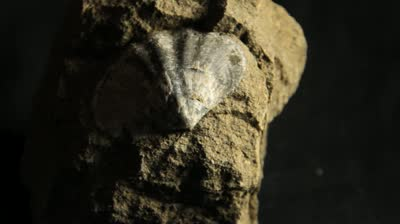
\includegraphics[height = 0.5\textheight, width = 0.4\textwidth, keepaspectratio = true]{figure/stock-brac1}\hspace{0.2\textwidth}%
    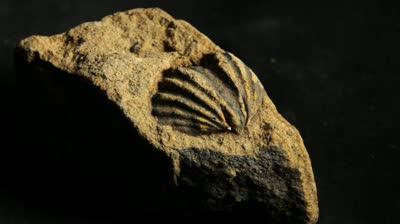
\includegraphics[height = 0.5\textheight, width = 0.4\textwidth, keepaspectratio = true]{figure/stock-brac2}\\[2em]
    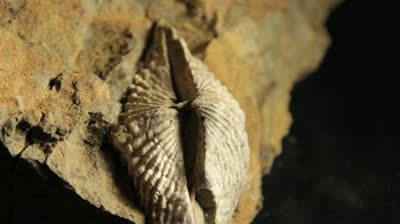
\includegraphics[height = 0.5\textheight, width = 0.4\textwidth, keepaspectratio = true]{figure/stock-brac3}\hspace{0.2\textwidth}%
    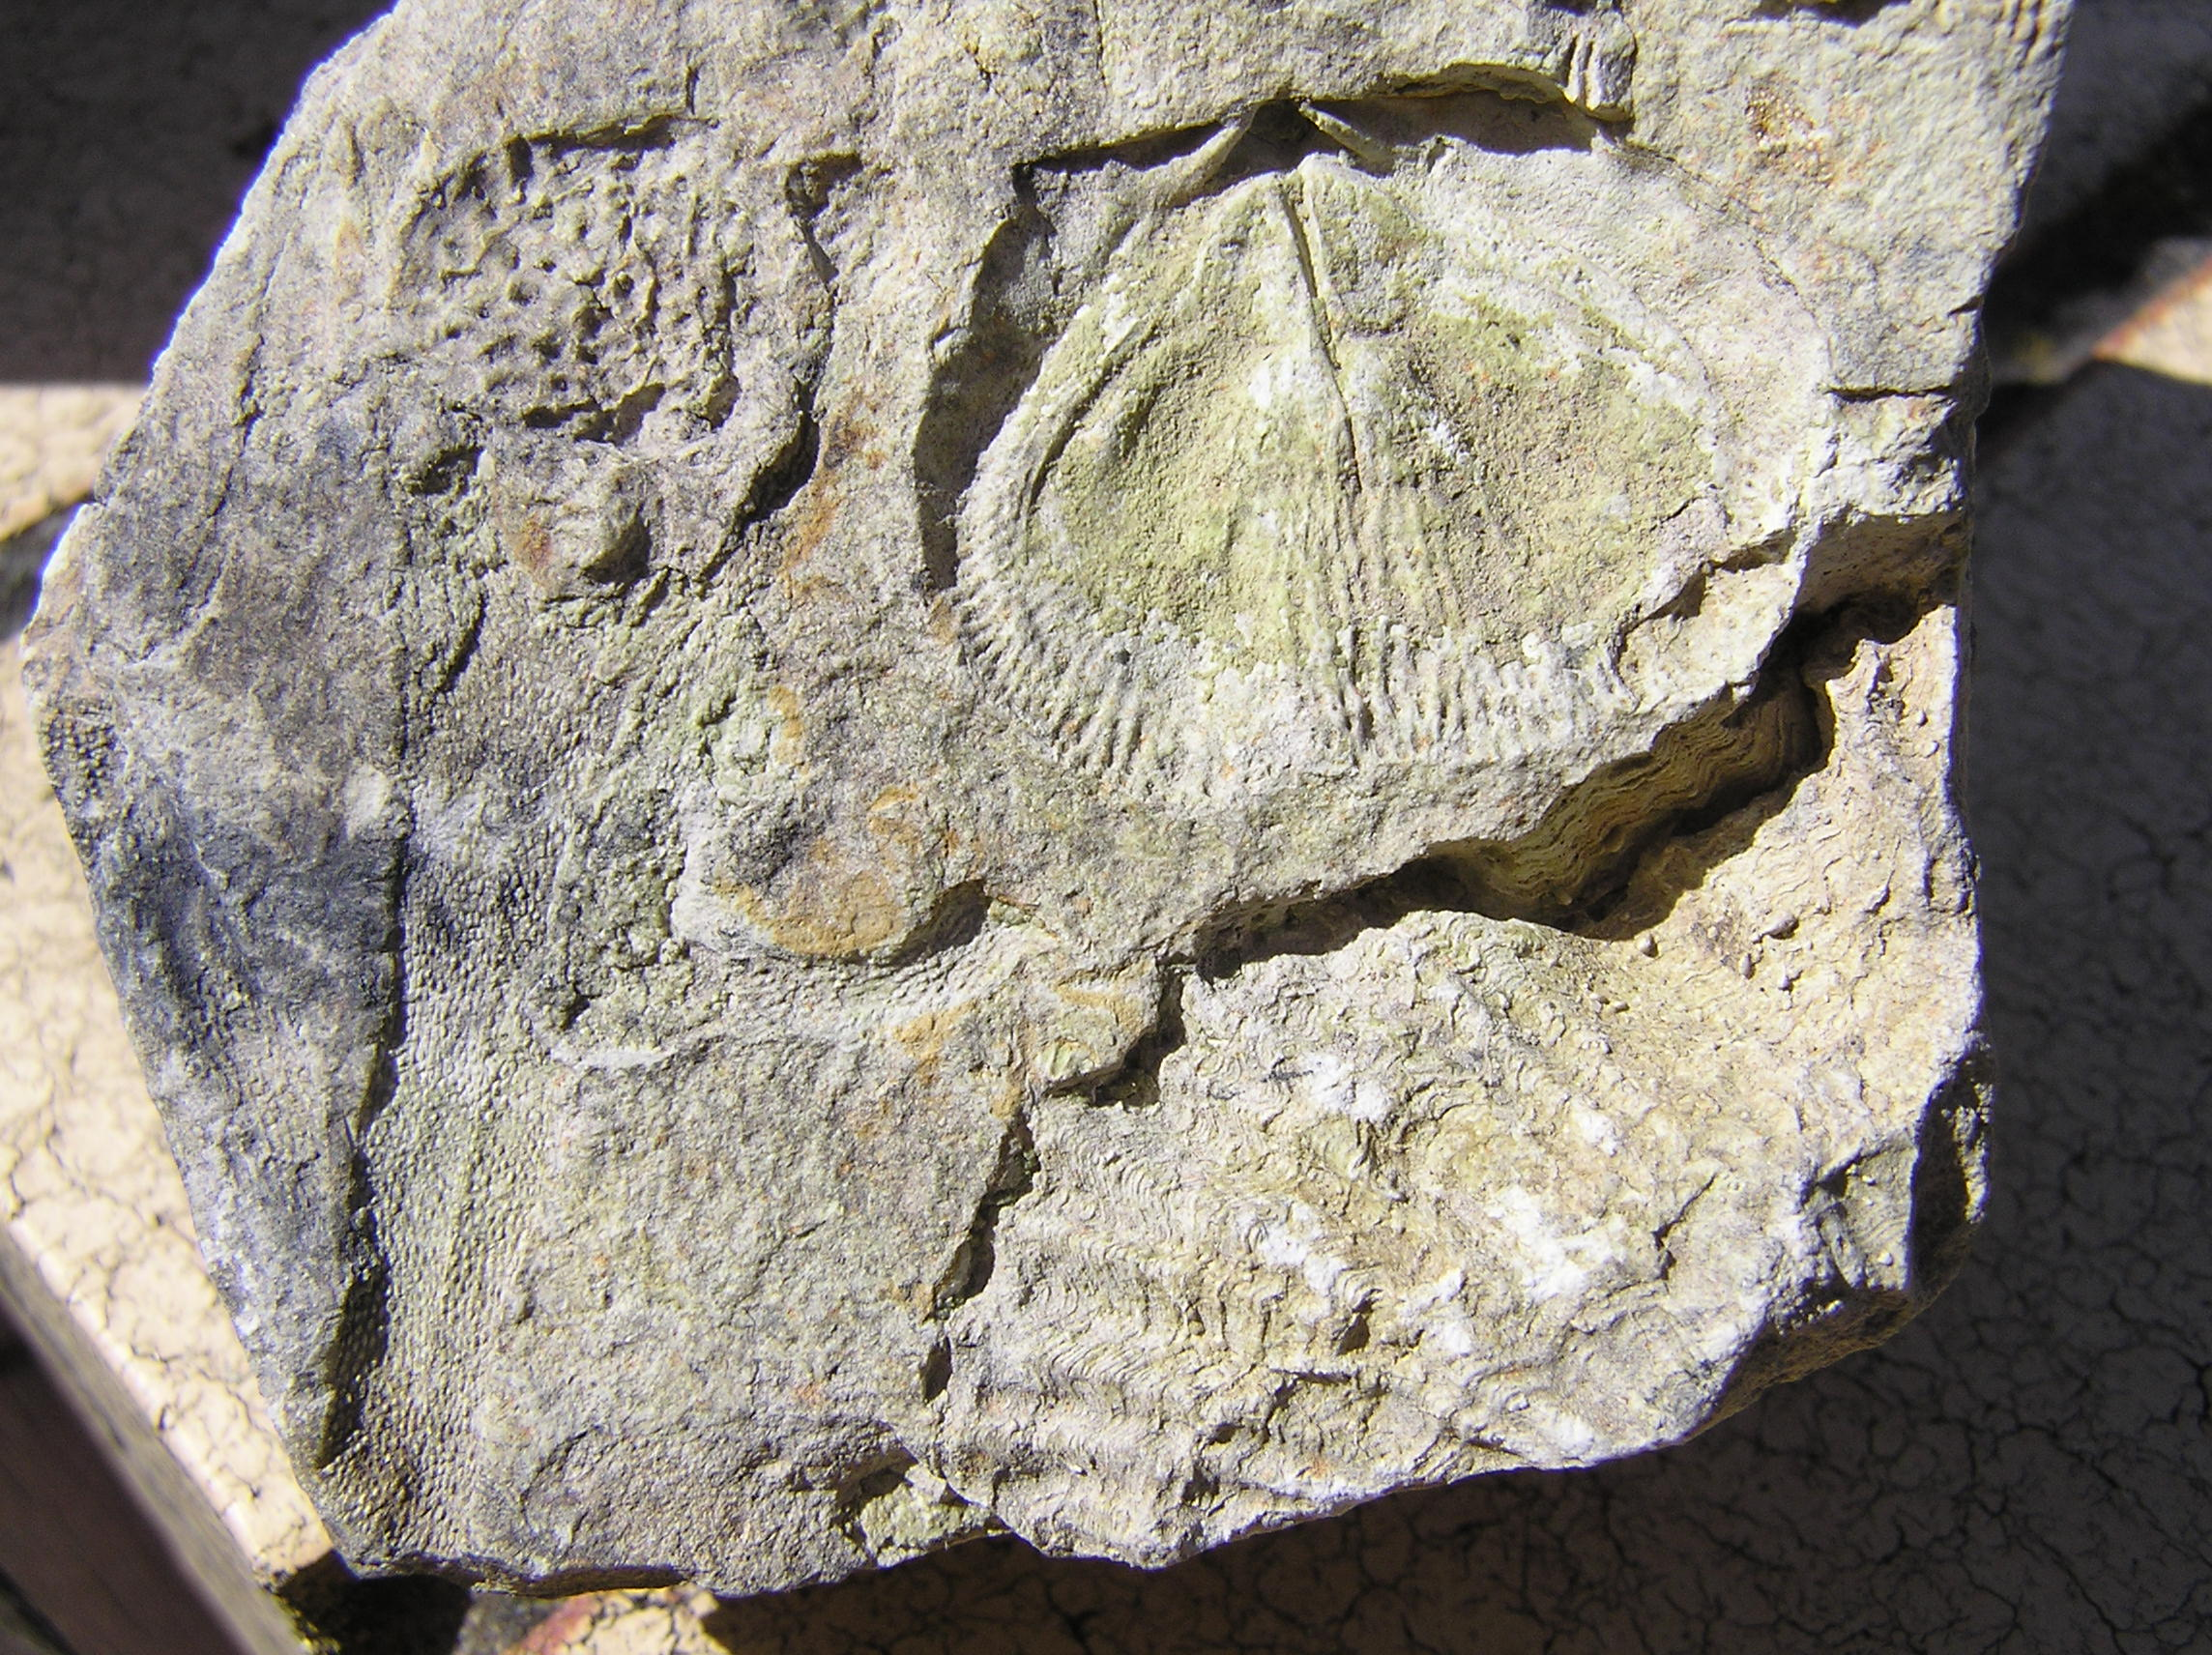
\includegraphics[height = 0.5\textheight, width = 0.4\textwidth, keepaspectratio = true]{figure/wiki_brac}\par

    \tiny{\attrib{Immersion Imagery, Shutterstock; Wikimedia}}
  \end{center}
\end{frame}


\begin{frame}
  \frametitle{System details}
  \begin{columns}
    \begin{column}{0.5\textwidth}
      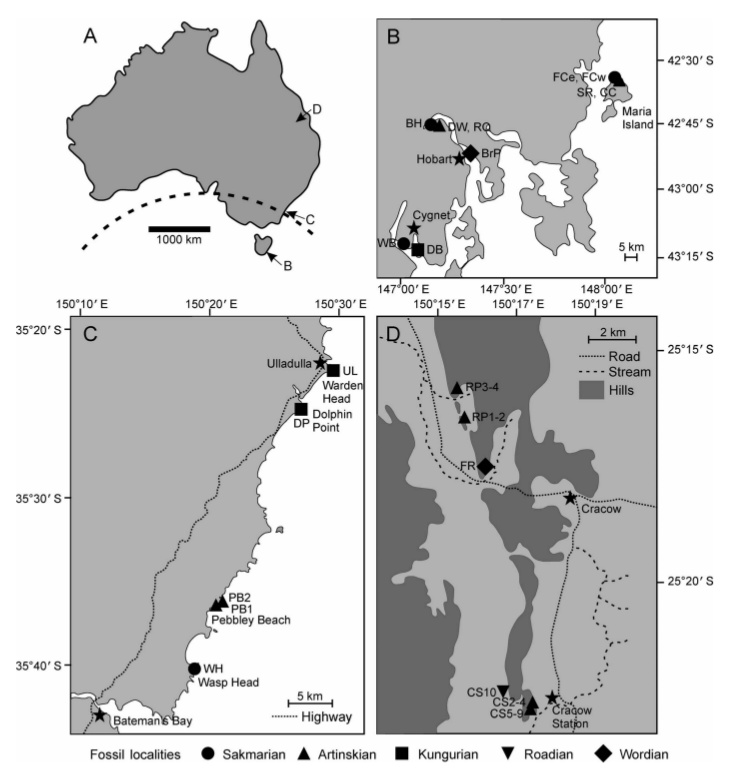
\includegraphics[height = 0.8\textheight, width = \textwidth, keepaspectratio = true]{figure/australia}

      \tiny{\attrib{Clapham and James 2008 \textit{Palaios}}}
    \end{column}
    \begin{column}{0.5\textwidth}
      \begin{itemize}
        \item Australian Permian
          \begin{itemize}
            \item range in/out taxa right censored
          \end{itemize}
        \item predictors 
          \begin{itemize}
            \item substrate probability 
            \item onshore/offshore probability
            \item body size (Payne \textit{et al.} 2014 \textit{Proc. B})
            \item occupancy (see Vilhena \textit{et al.} 2014 \textit{Nature Com.})
          \end{itemize}
      \end{itemize}
    \end{column}
  \end{columns}
\end{frame}


\begin{frame}
  \frametitle{Survival analysis: constant extinction}

  \begin{center}
    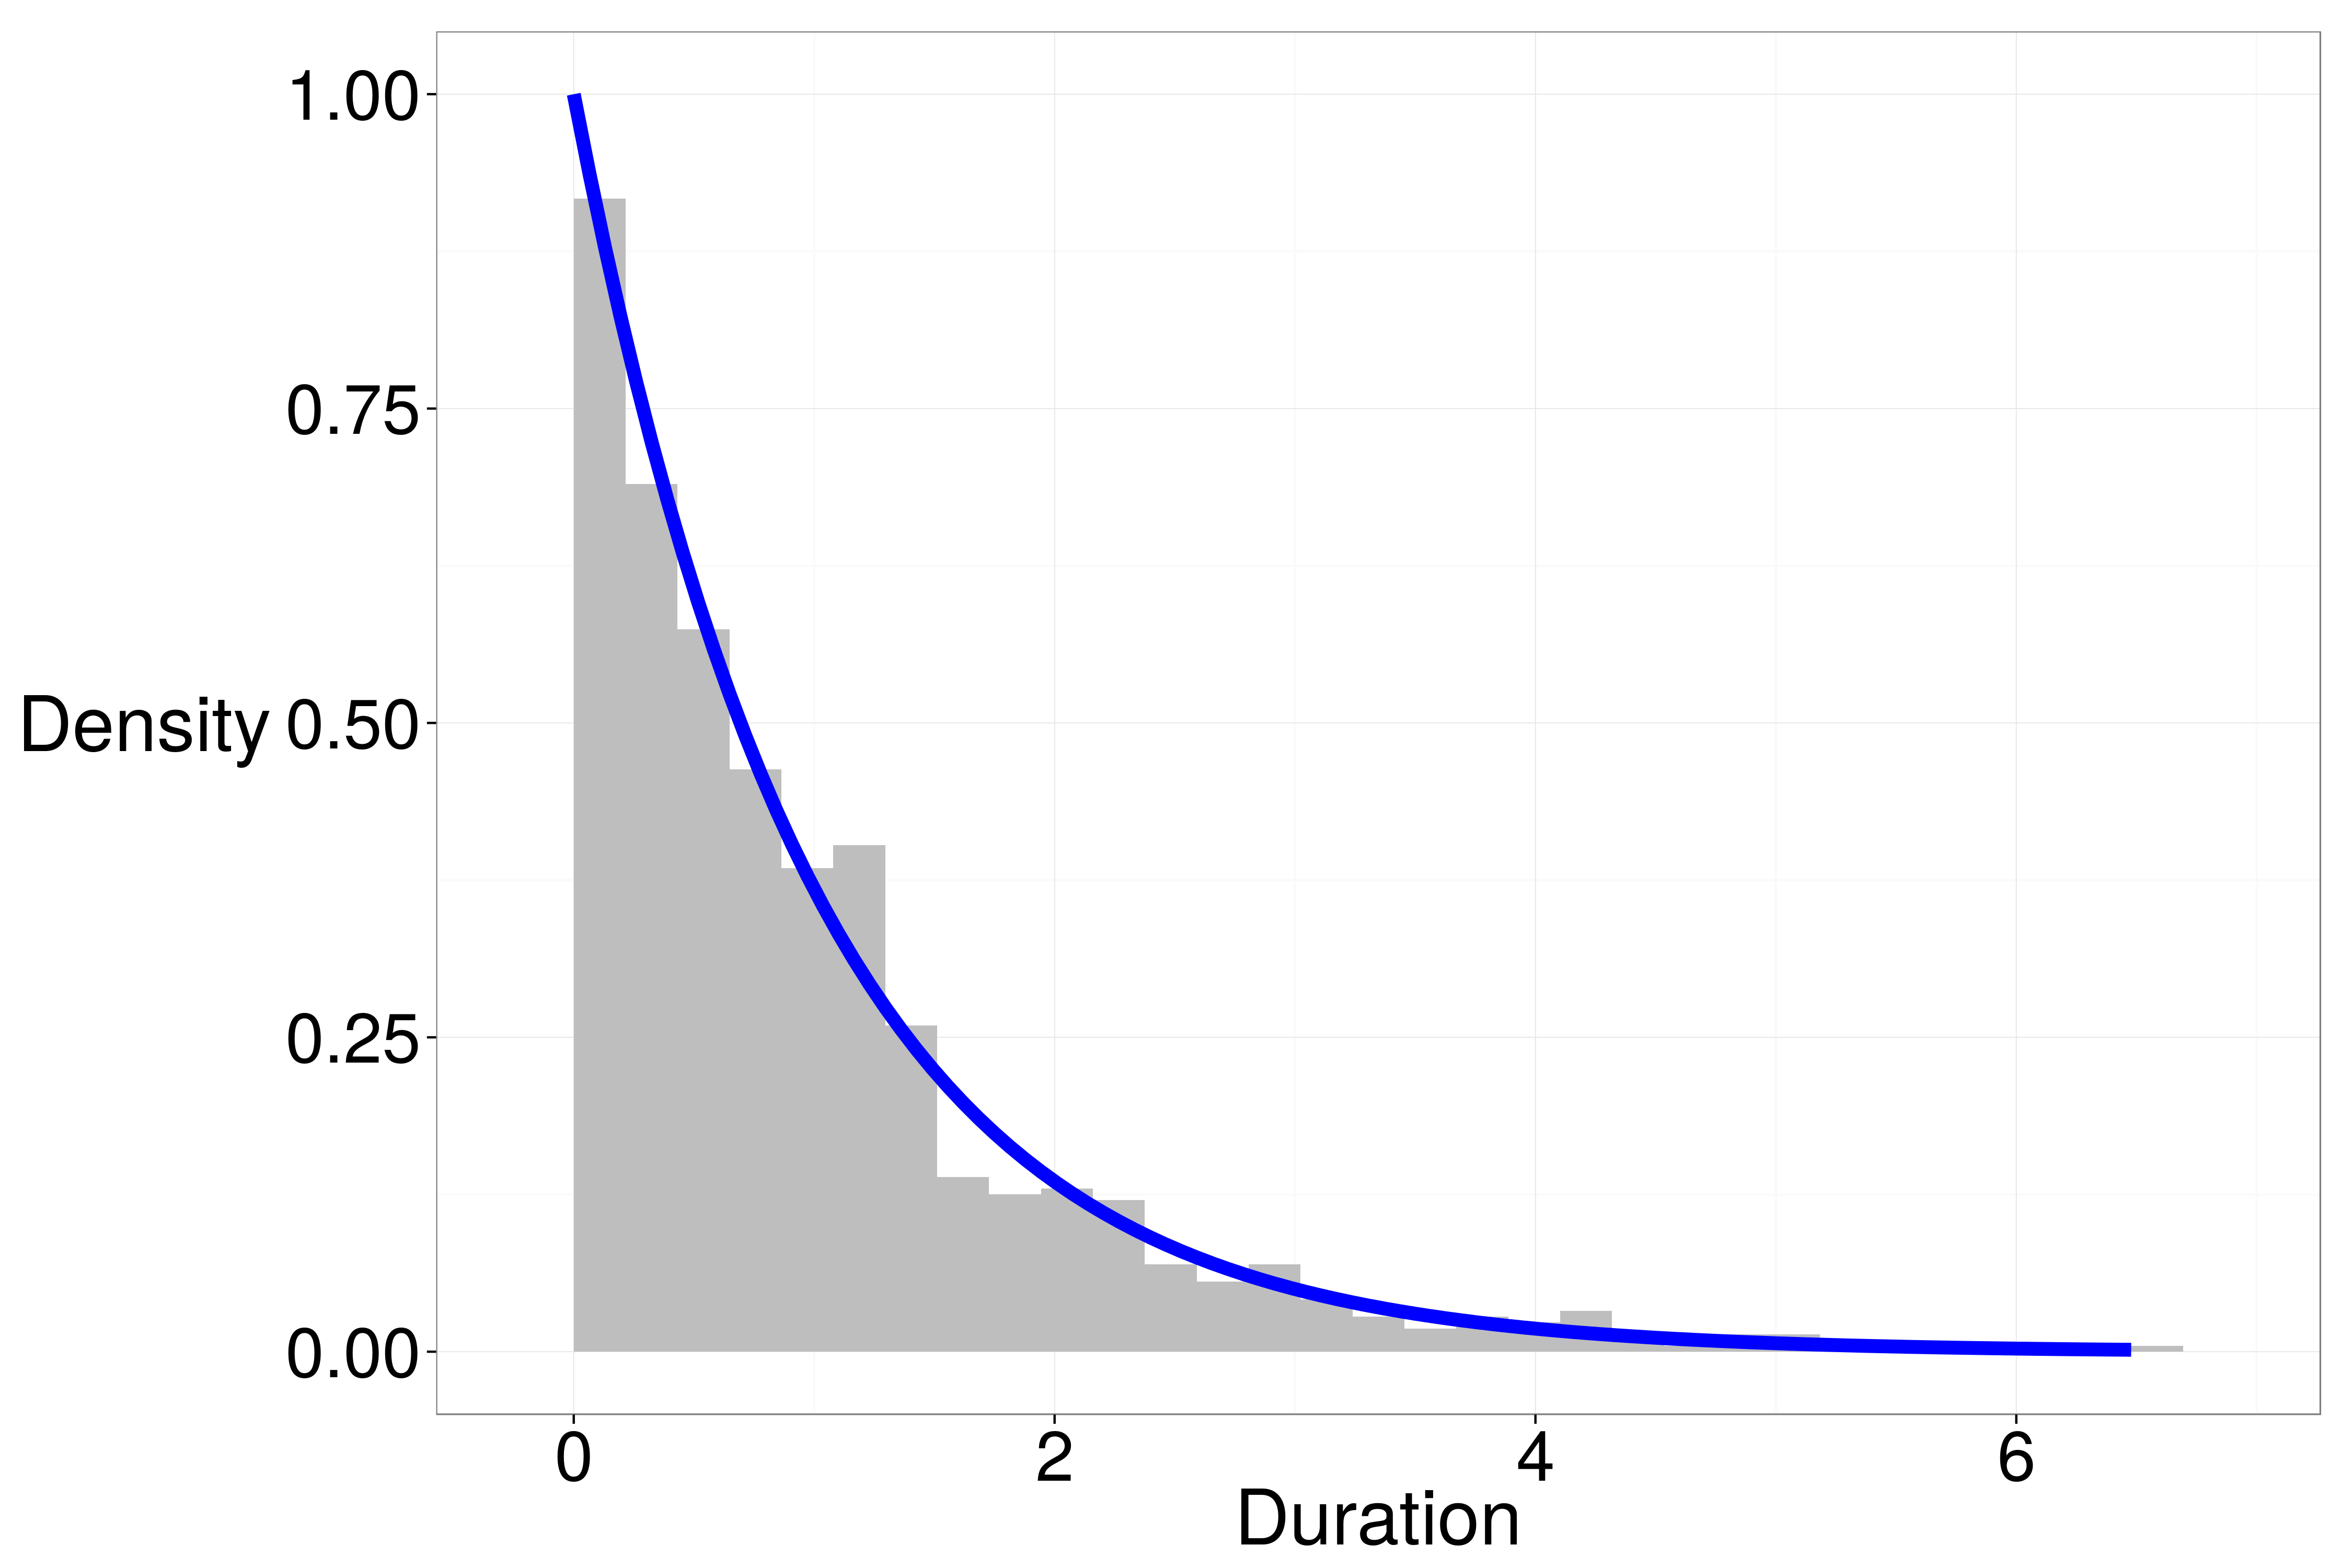
\includegraphics[height = 0.4\textheight, width = \textwidth, keepaspectratio = true]{figure/dur_exp}

    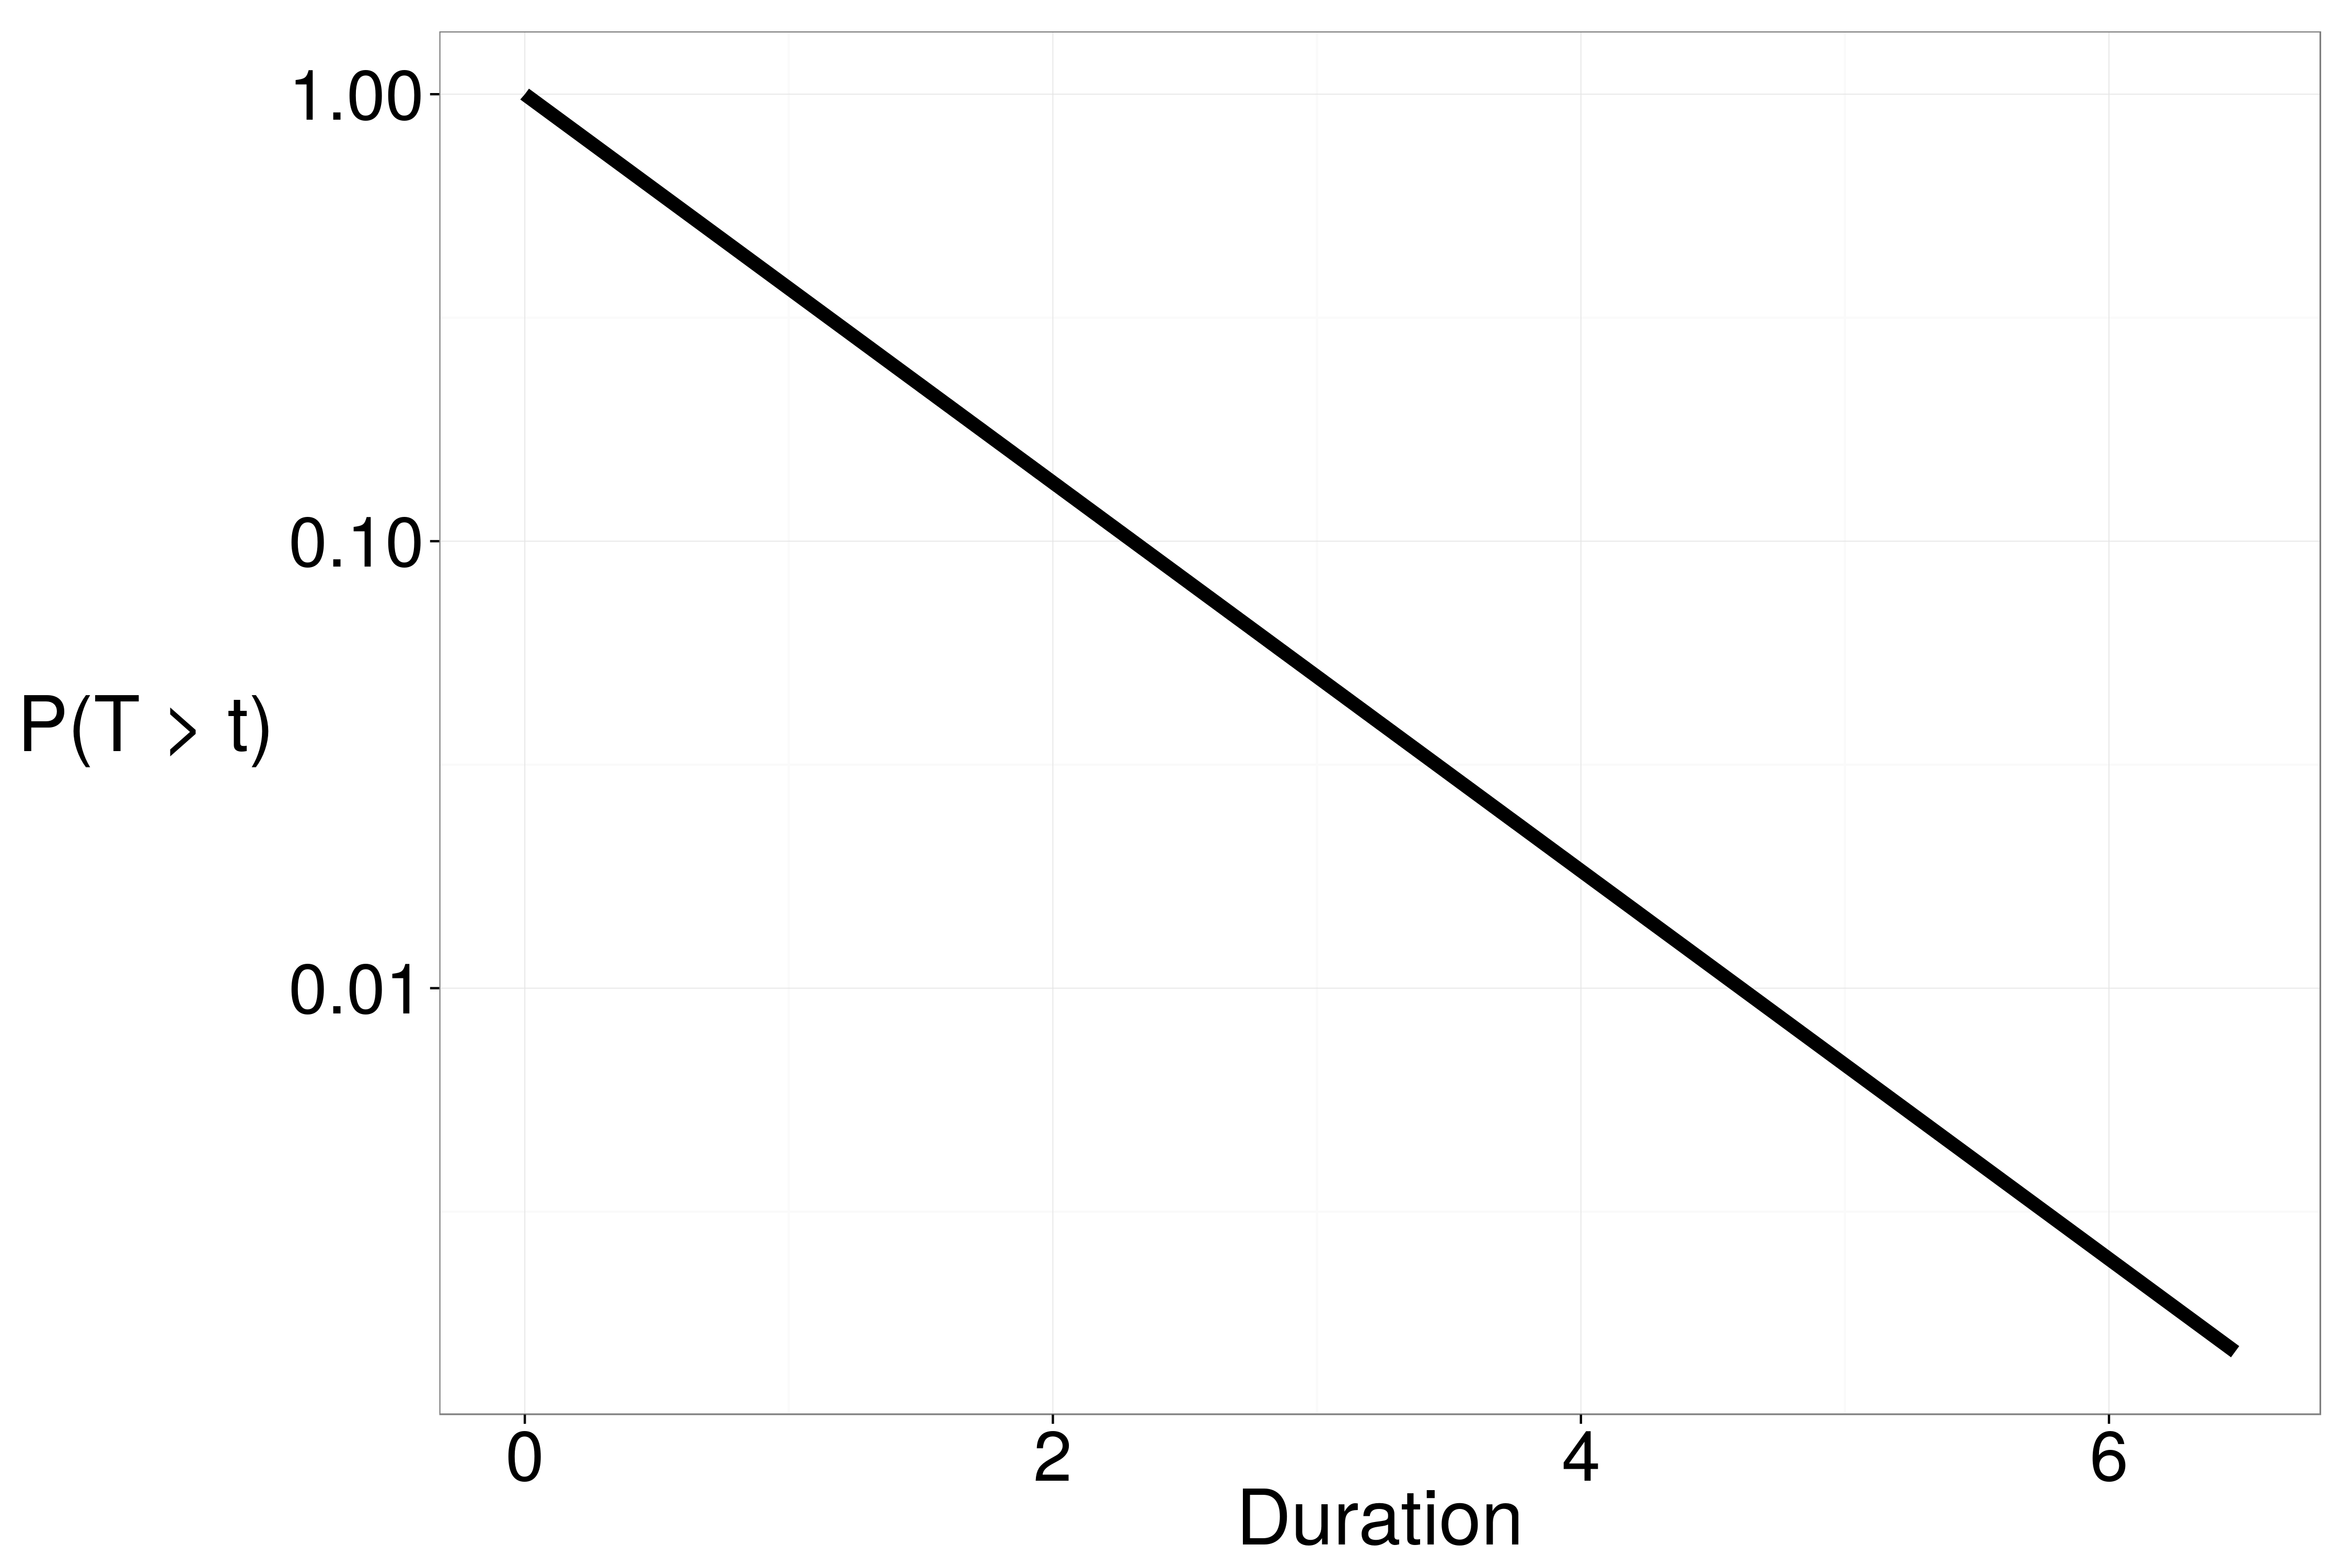
\includegraphics[height = 0.6\textheight, width = 0.5\textwidth, keepaspectratio = true]{figure/sur_exp}
    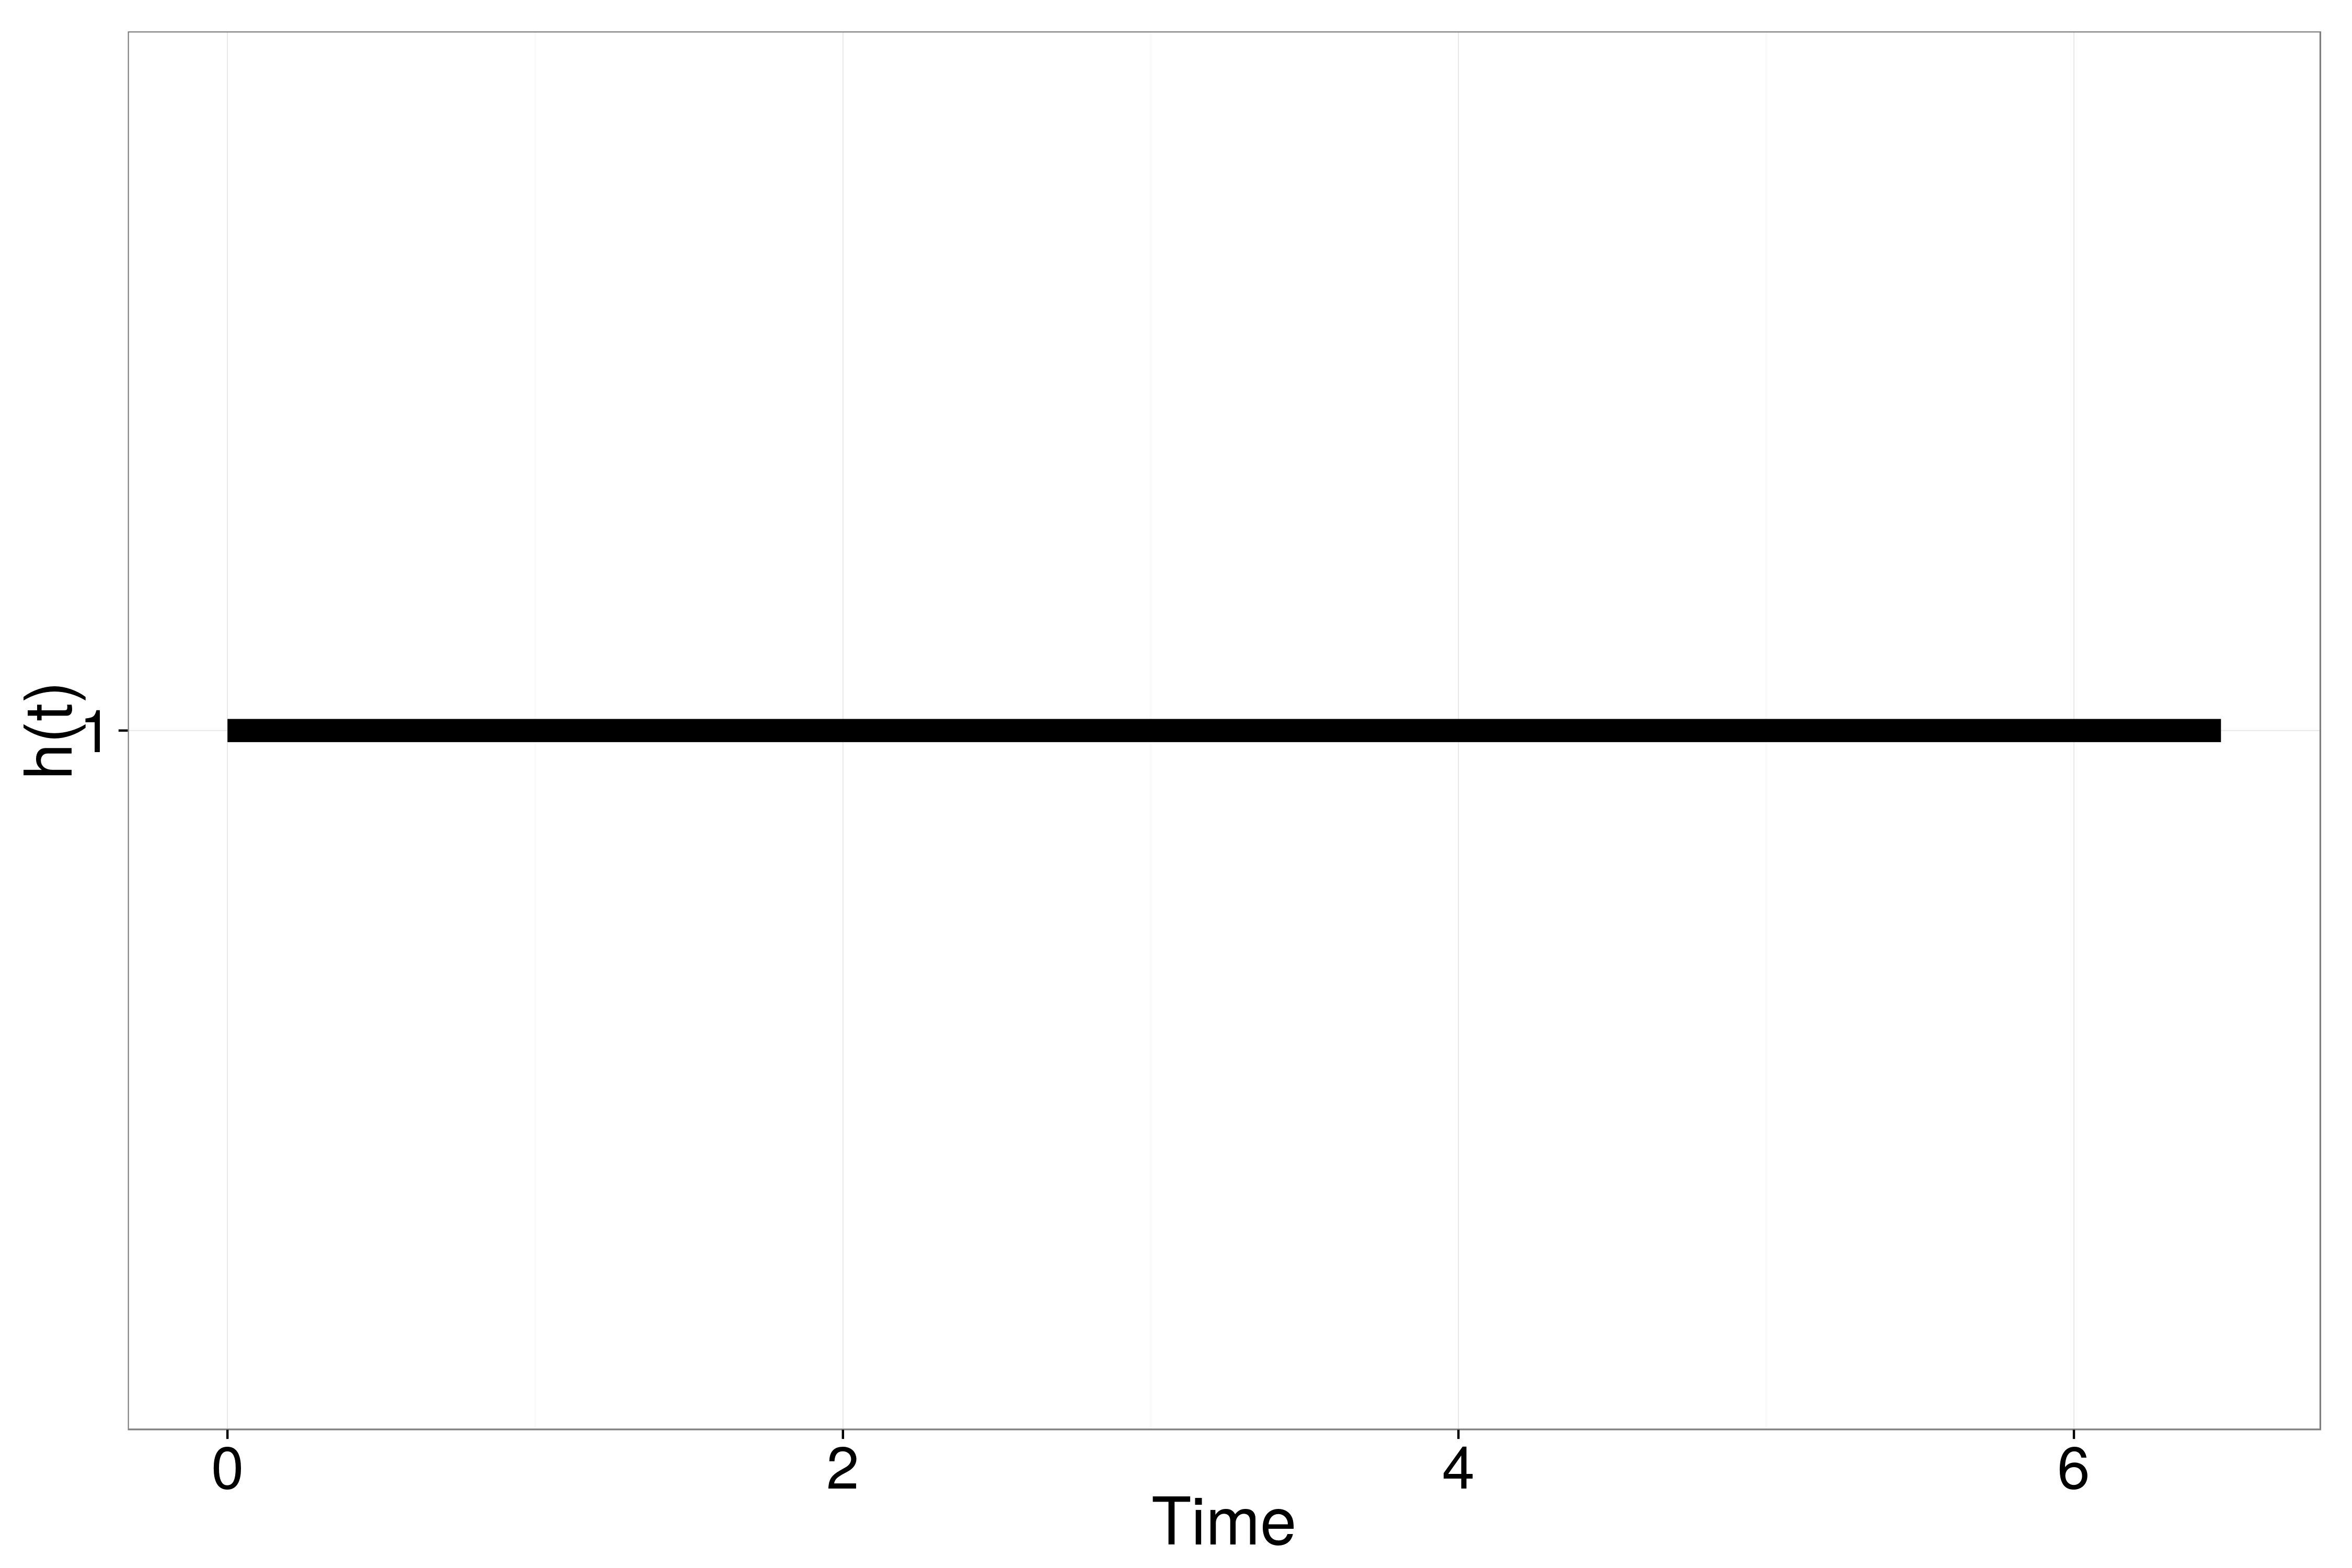
\includegraphics[height = 0.6\textheight, width = 0.5\textwidth, keepaspectratio = true]{figure/haz_exp}
  \end{center}
\end{frame}

\begin{frame}
  \frametitle{Survival analysis: decelerating (k \(<\) 1)}

  \begin{center}
    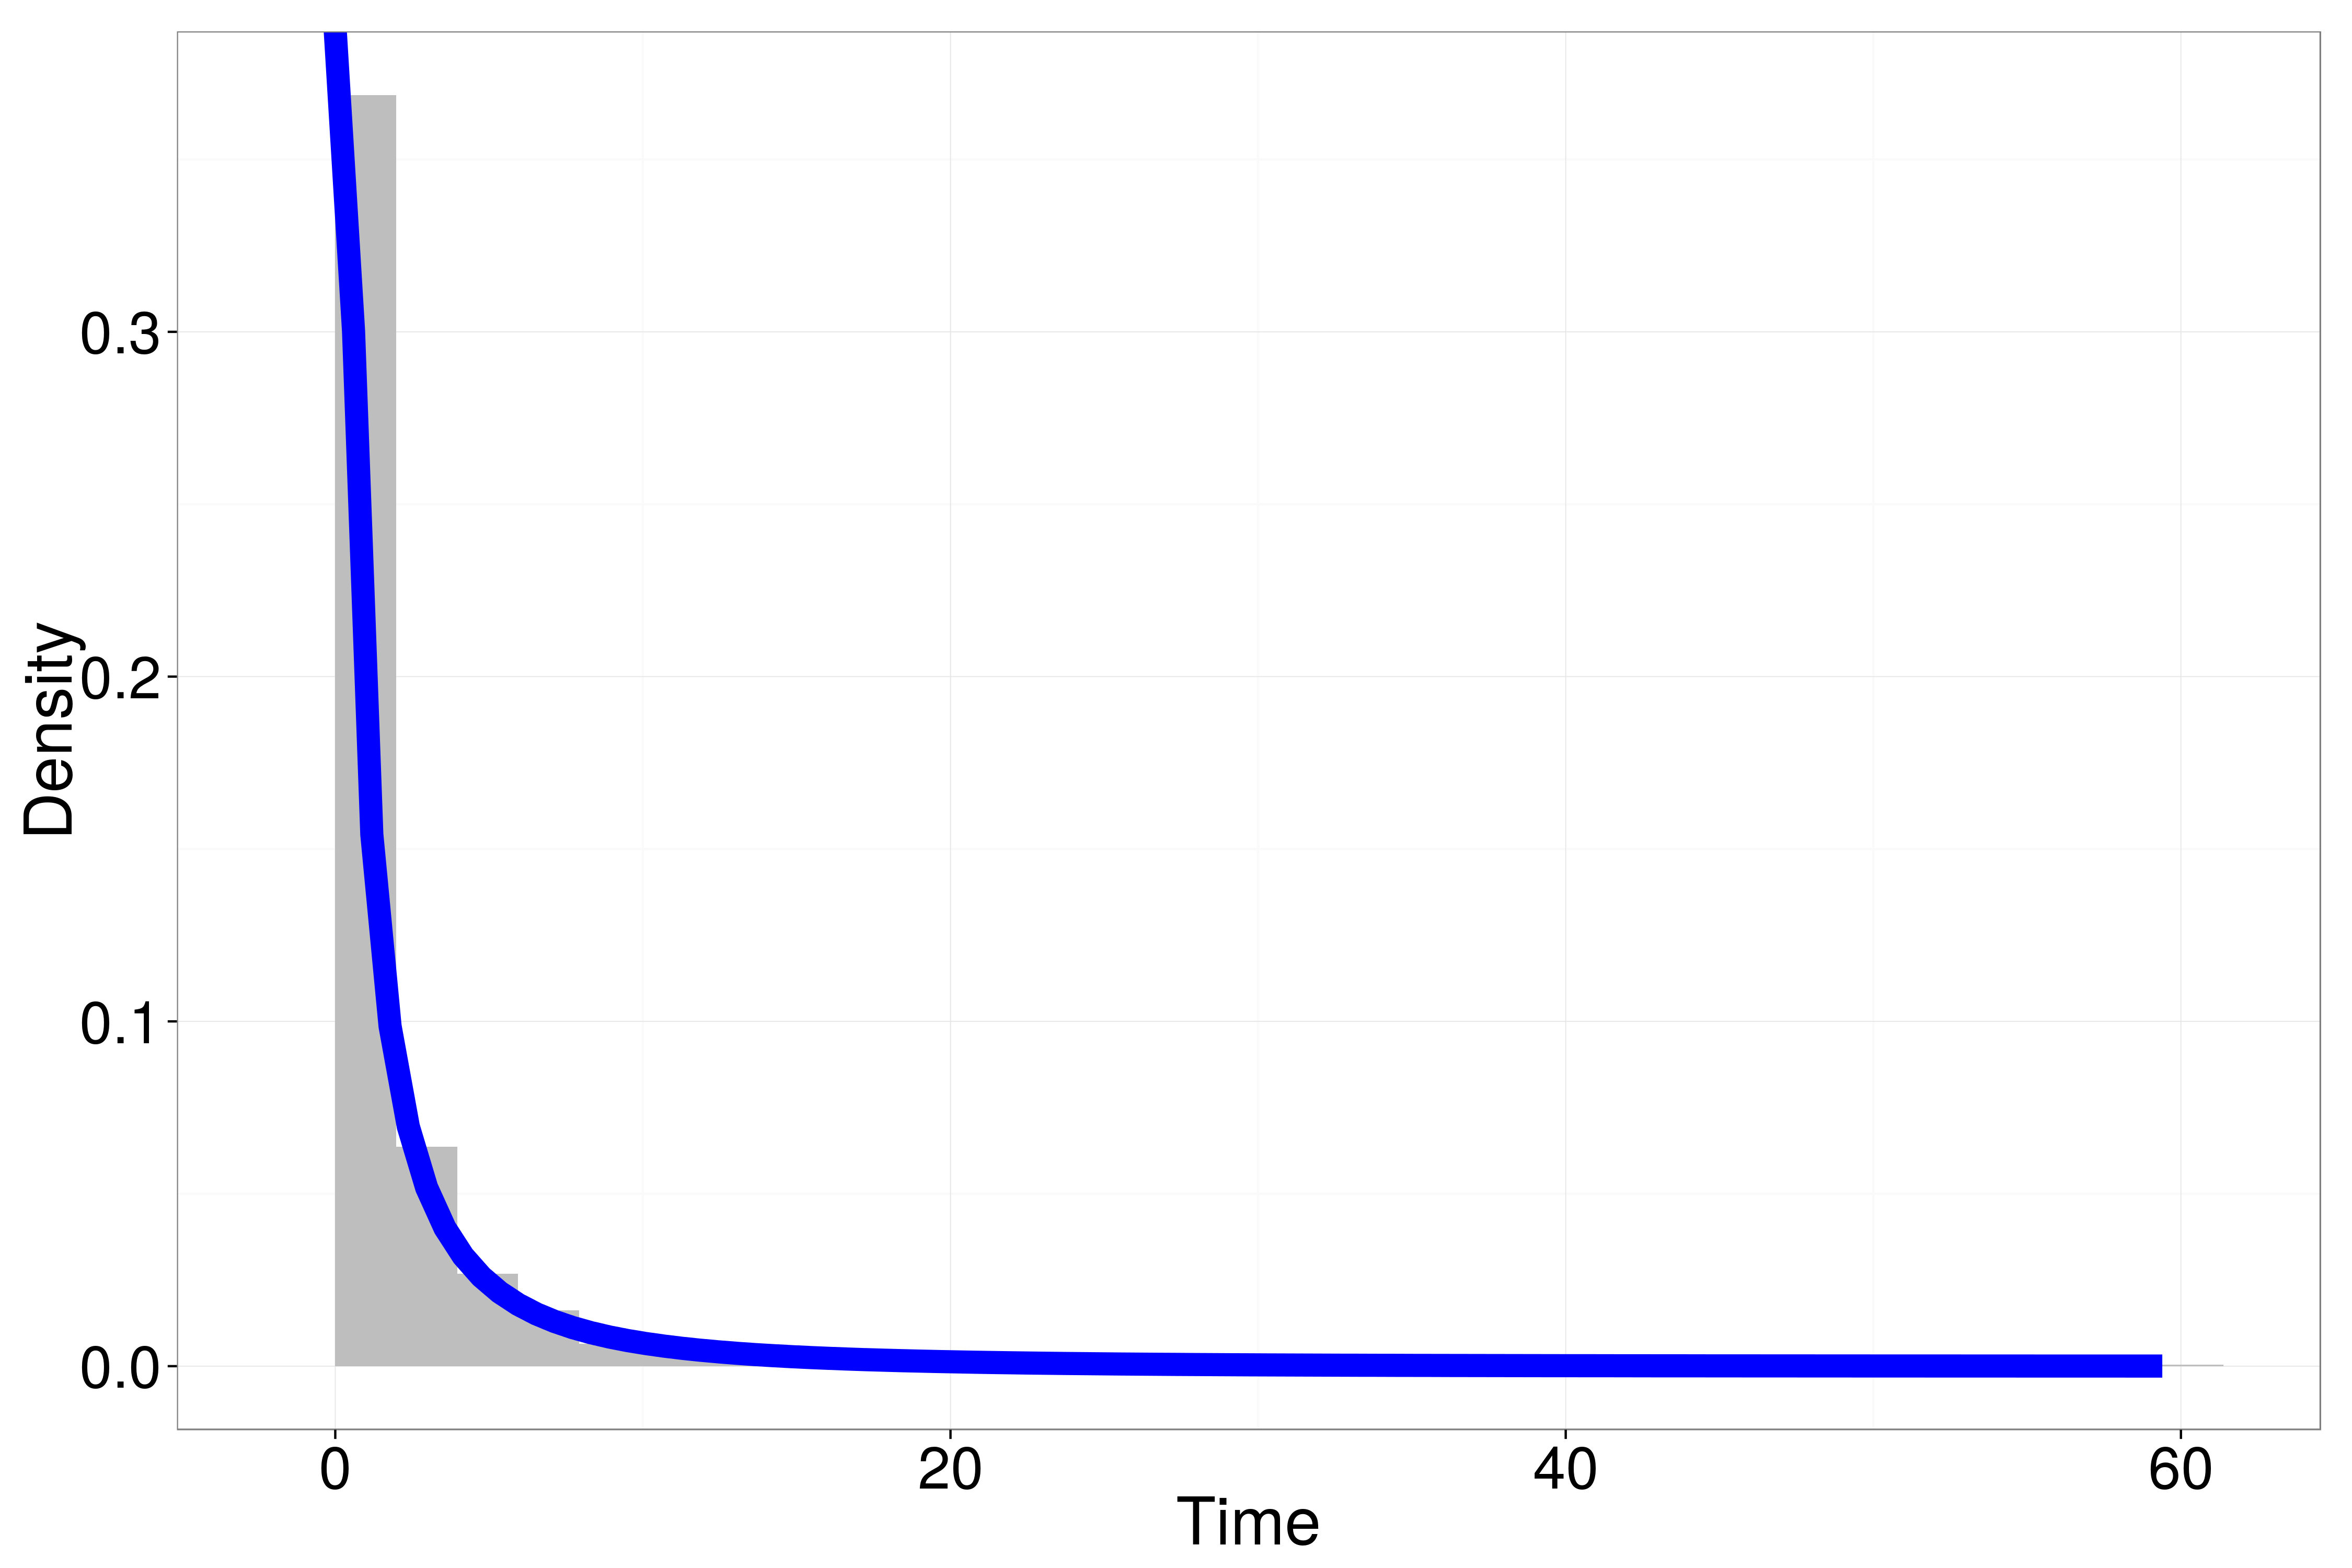
\includegraphics[height = 0.4\textheight, width = \textwidth, keepaspectratio = true]{figure/dur_dec}

    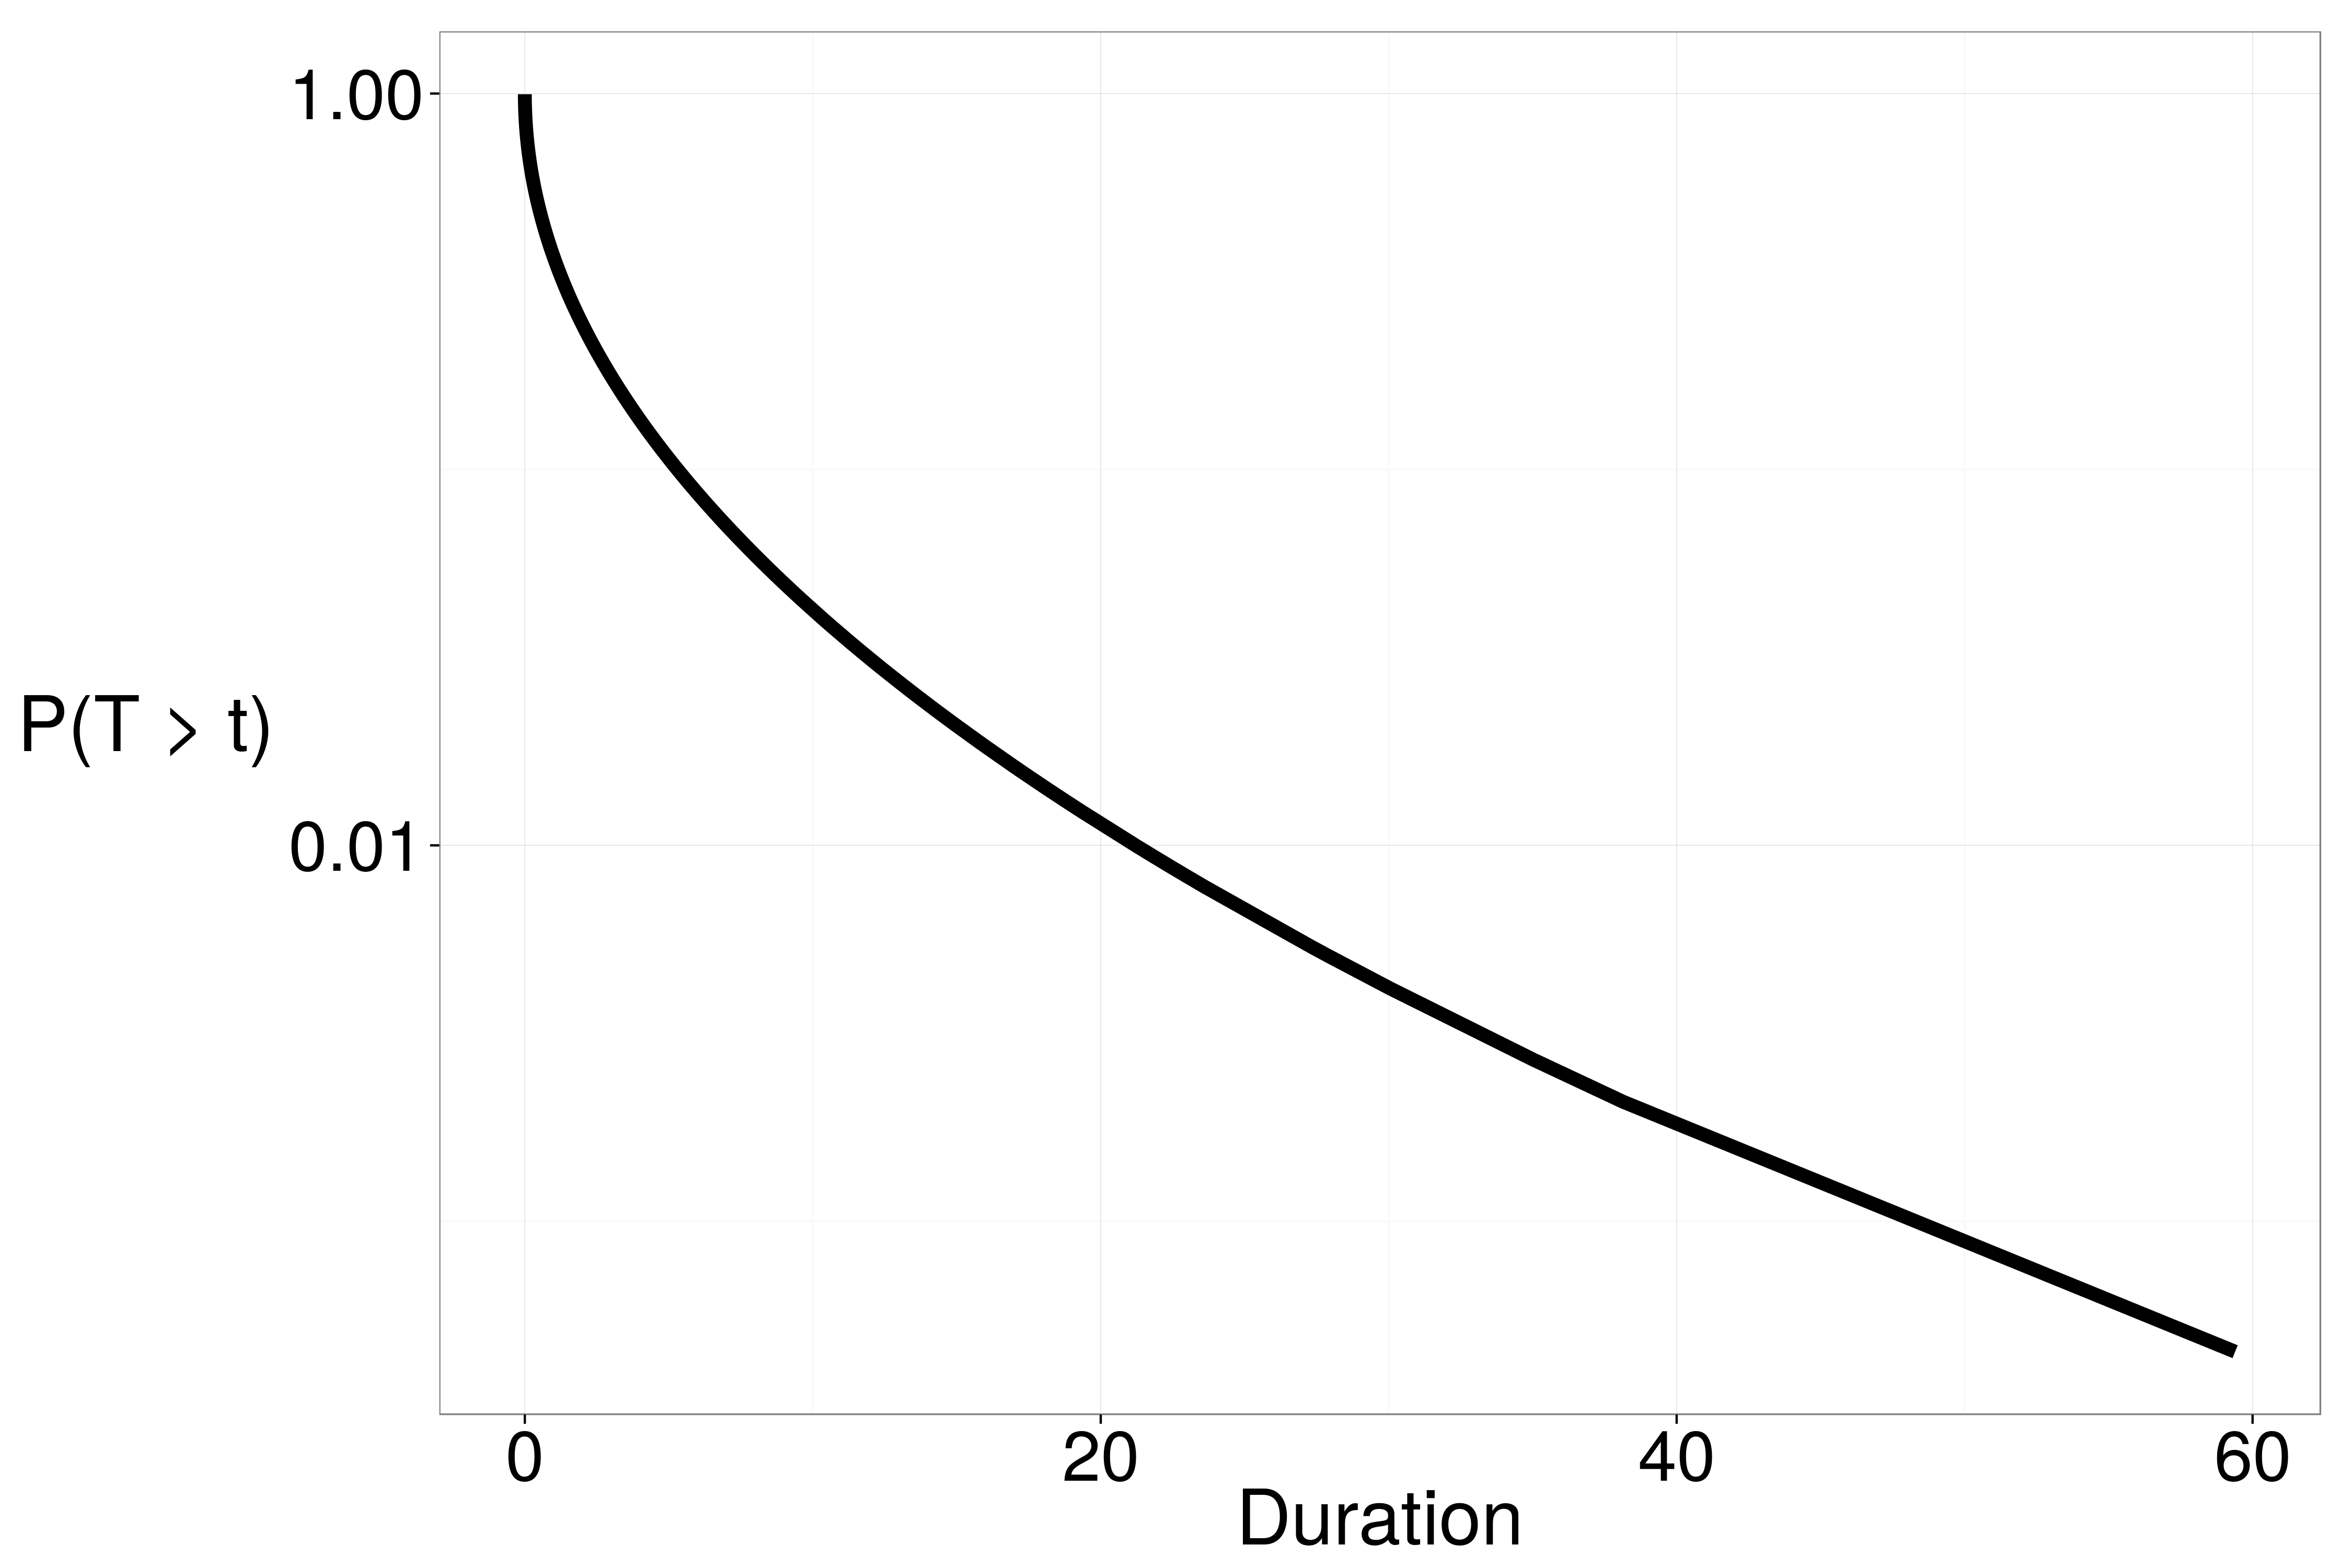
\includegraphics[height = 0.6\textheight, width = 0.5\textwidth, keepaspectratio = true]{figure/sur_dec}
    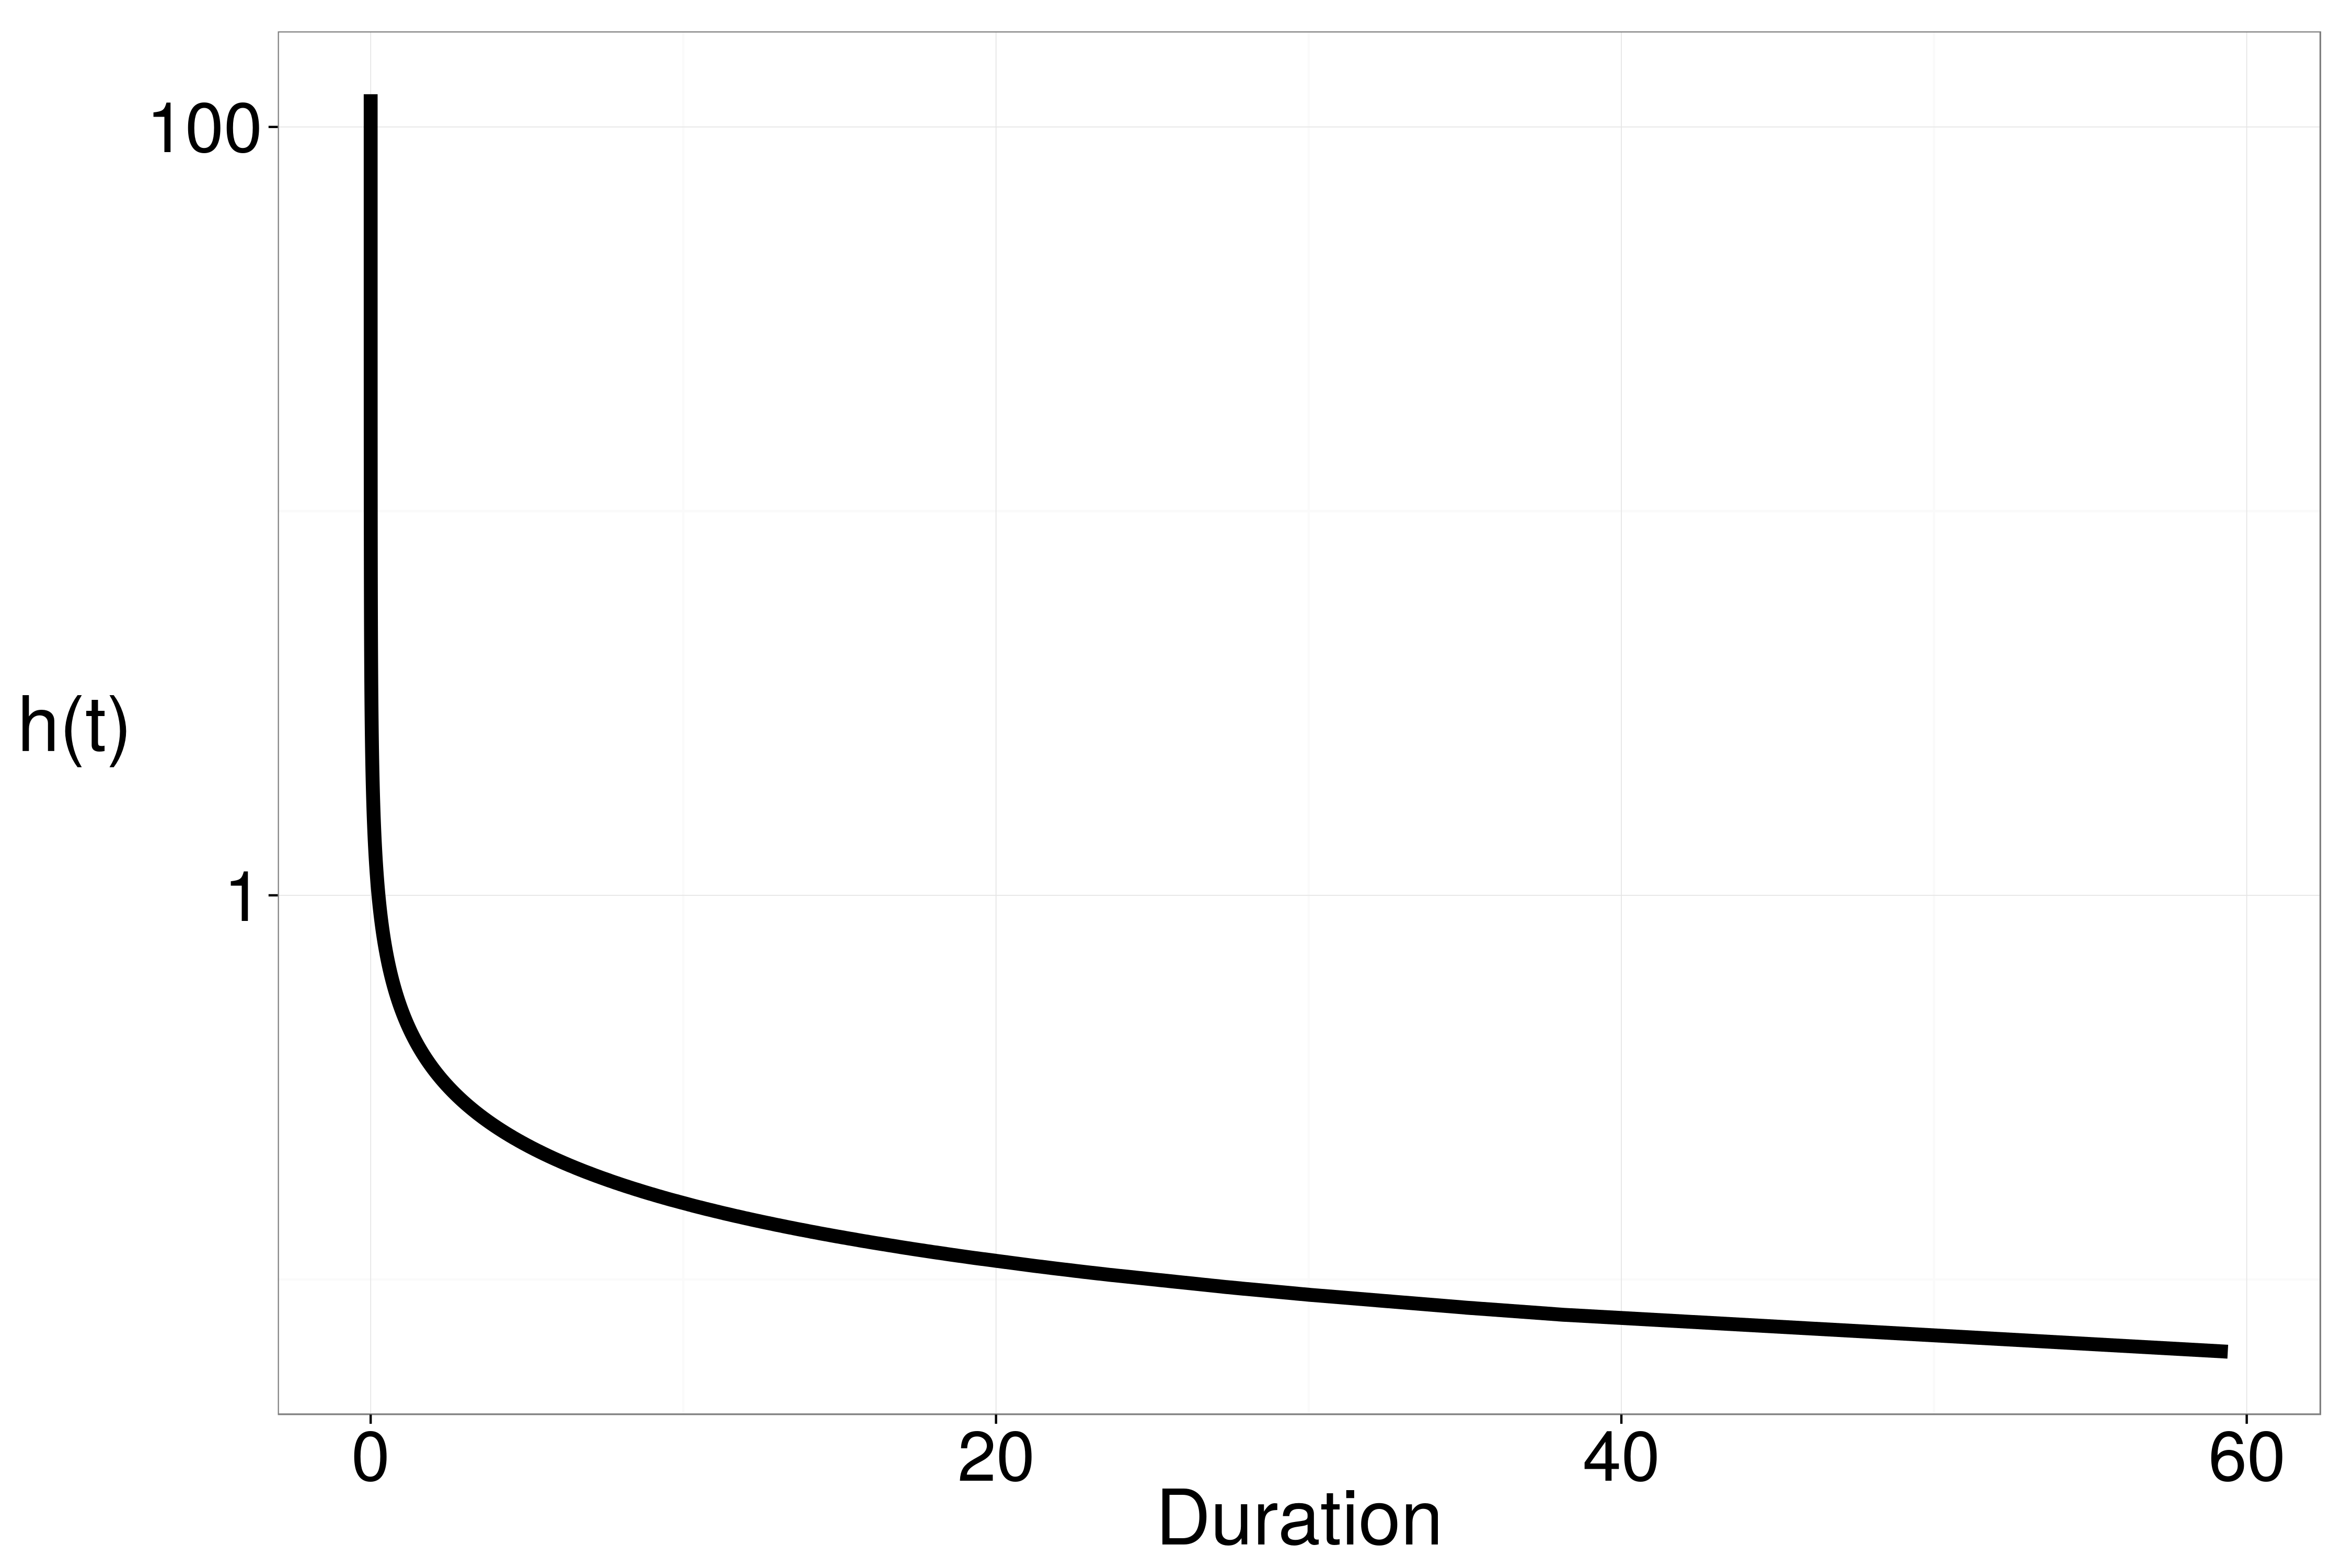
\includegraphics[height = 0.6\textheight, width = 0.5\textwidth, keepaspectratio = true]{figure/haz_dec}
  \end{center}
\end{frame}

\begin{frame}
  \frametitle{Survival analysis: accelerating (k \(>\) 1)}

  \begin{center}
    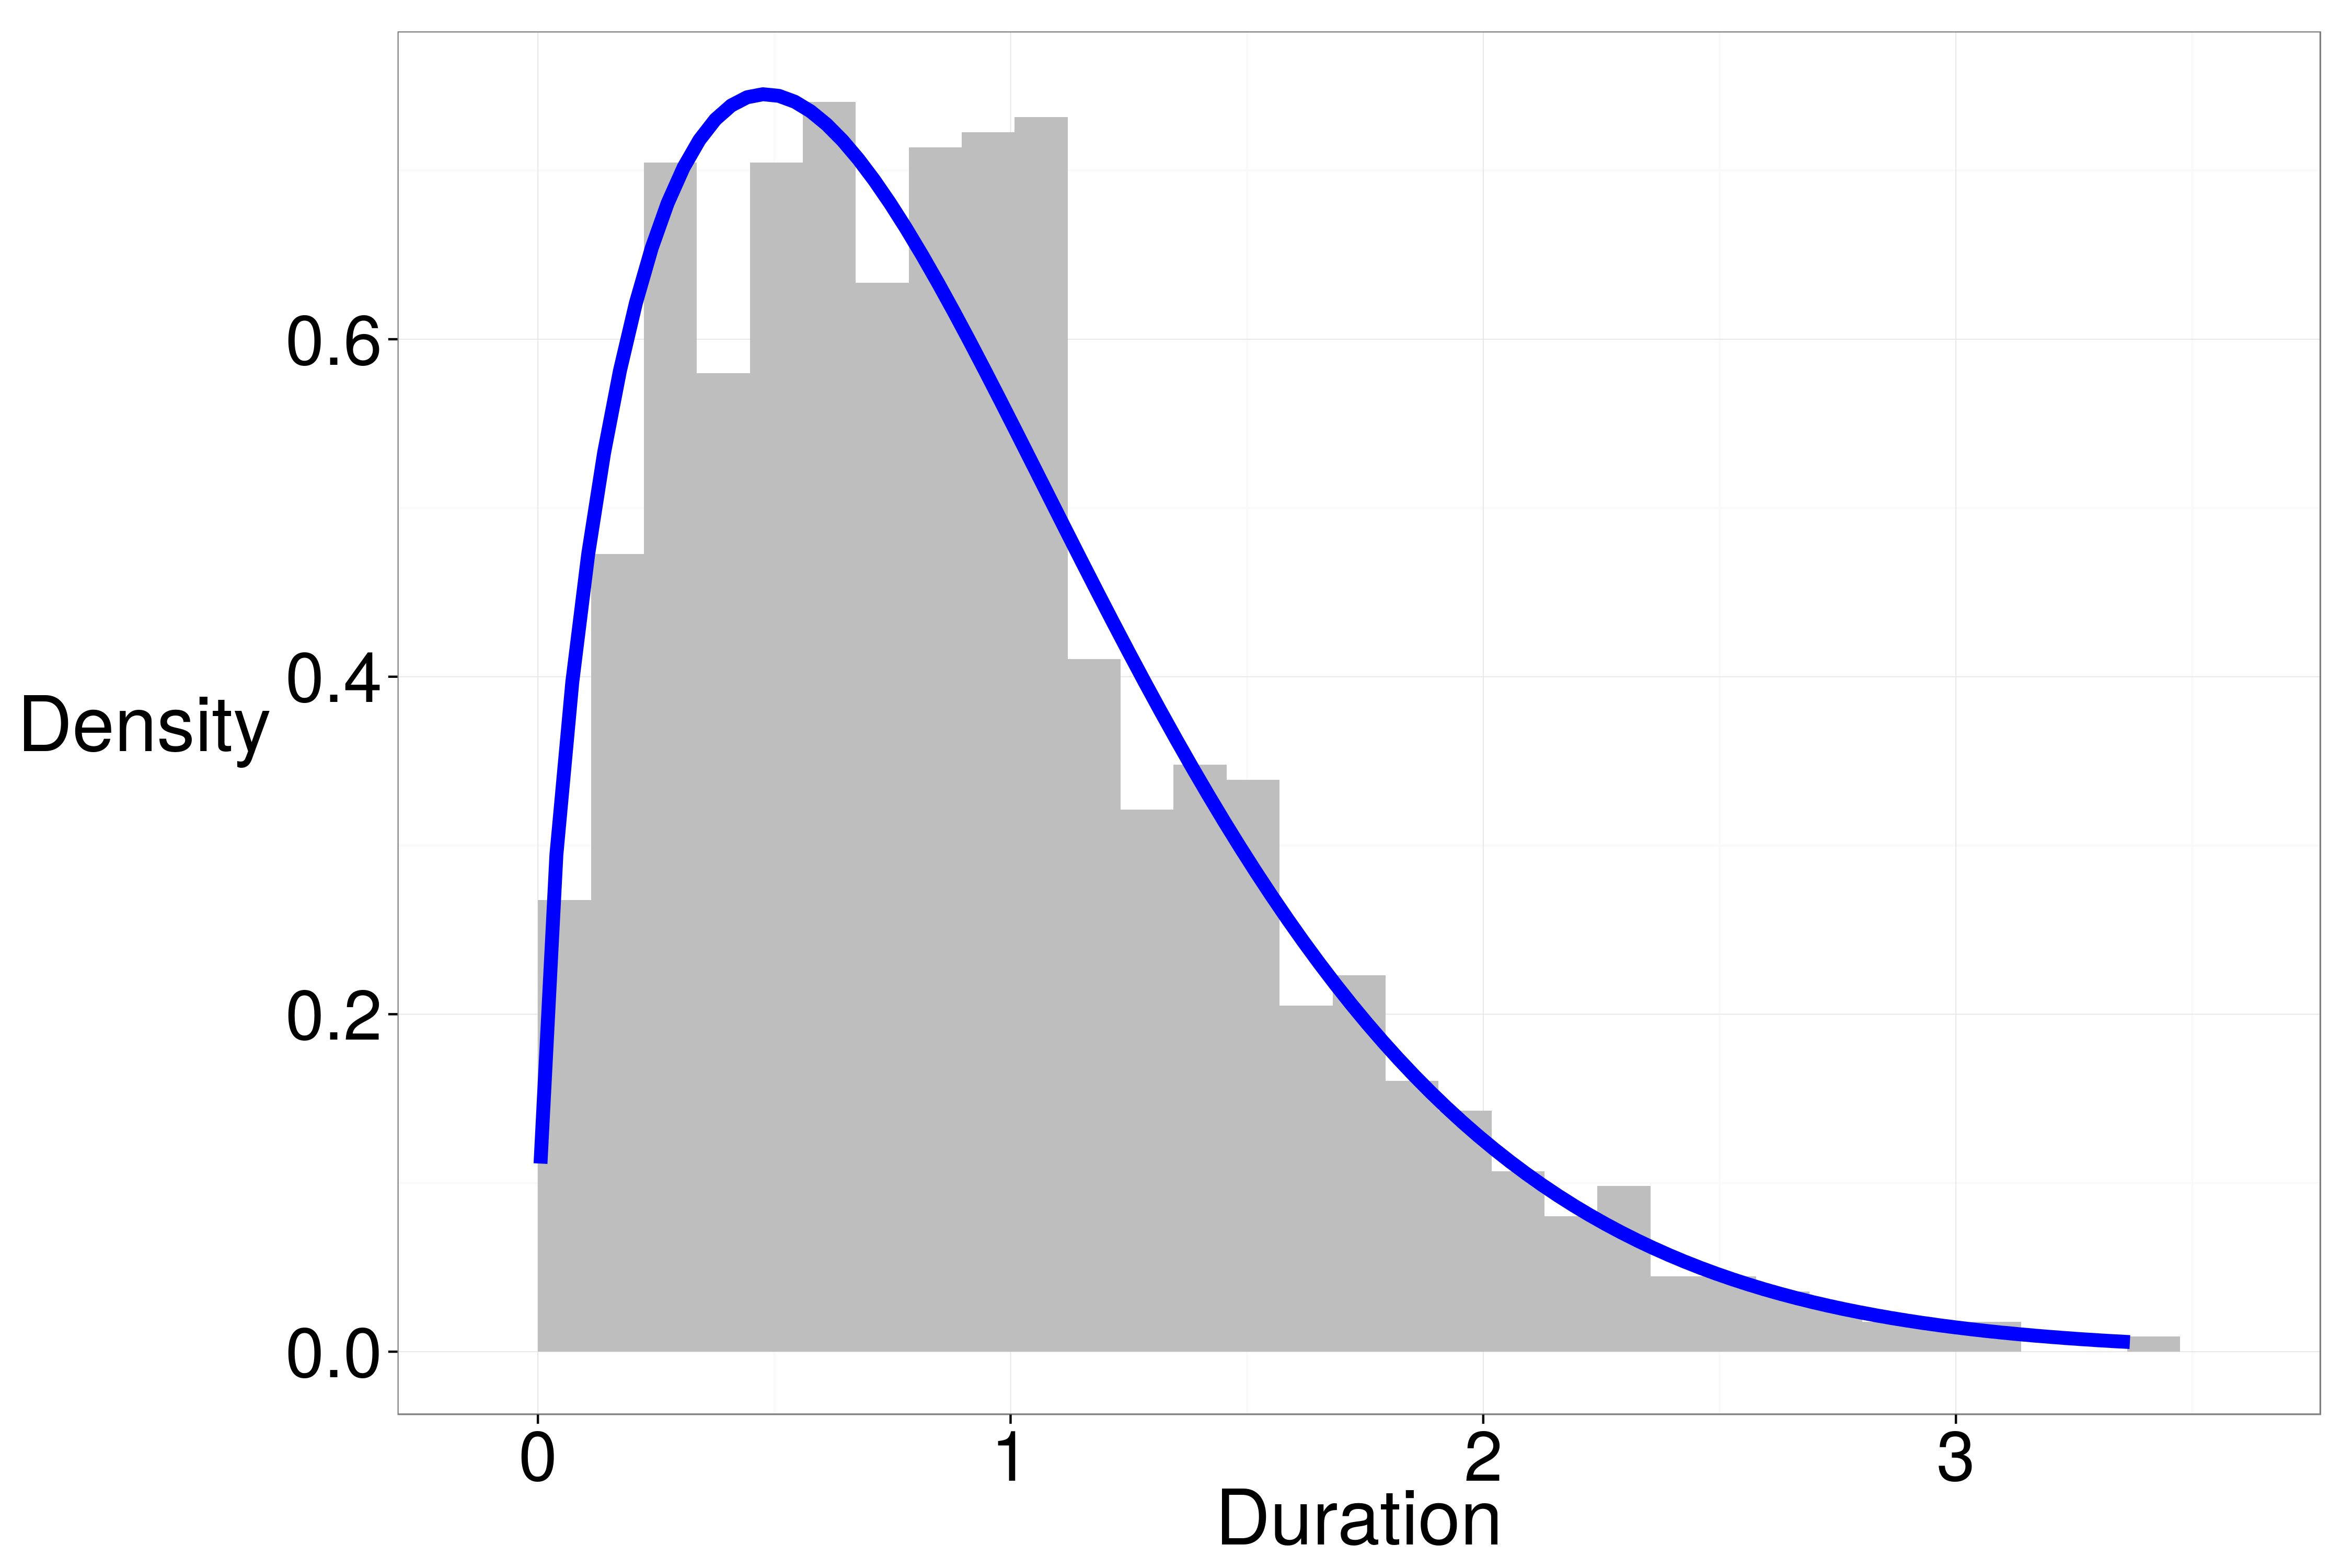
\includegraphics[height = 0.4\textheight, width = \textwidth, keepaspectratio = true]{figure/dur_acc}

    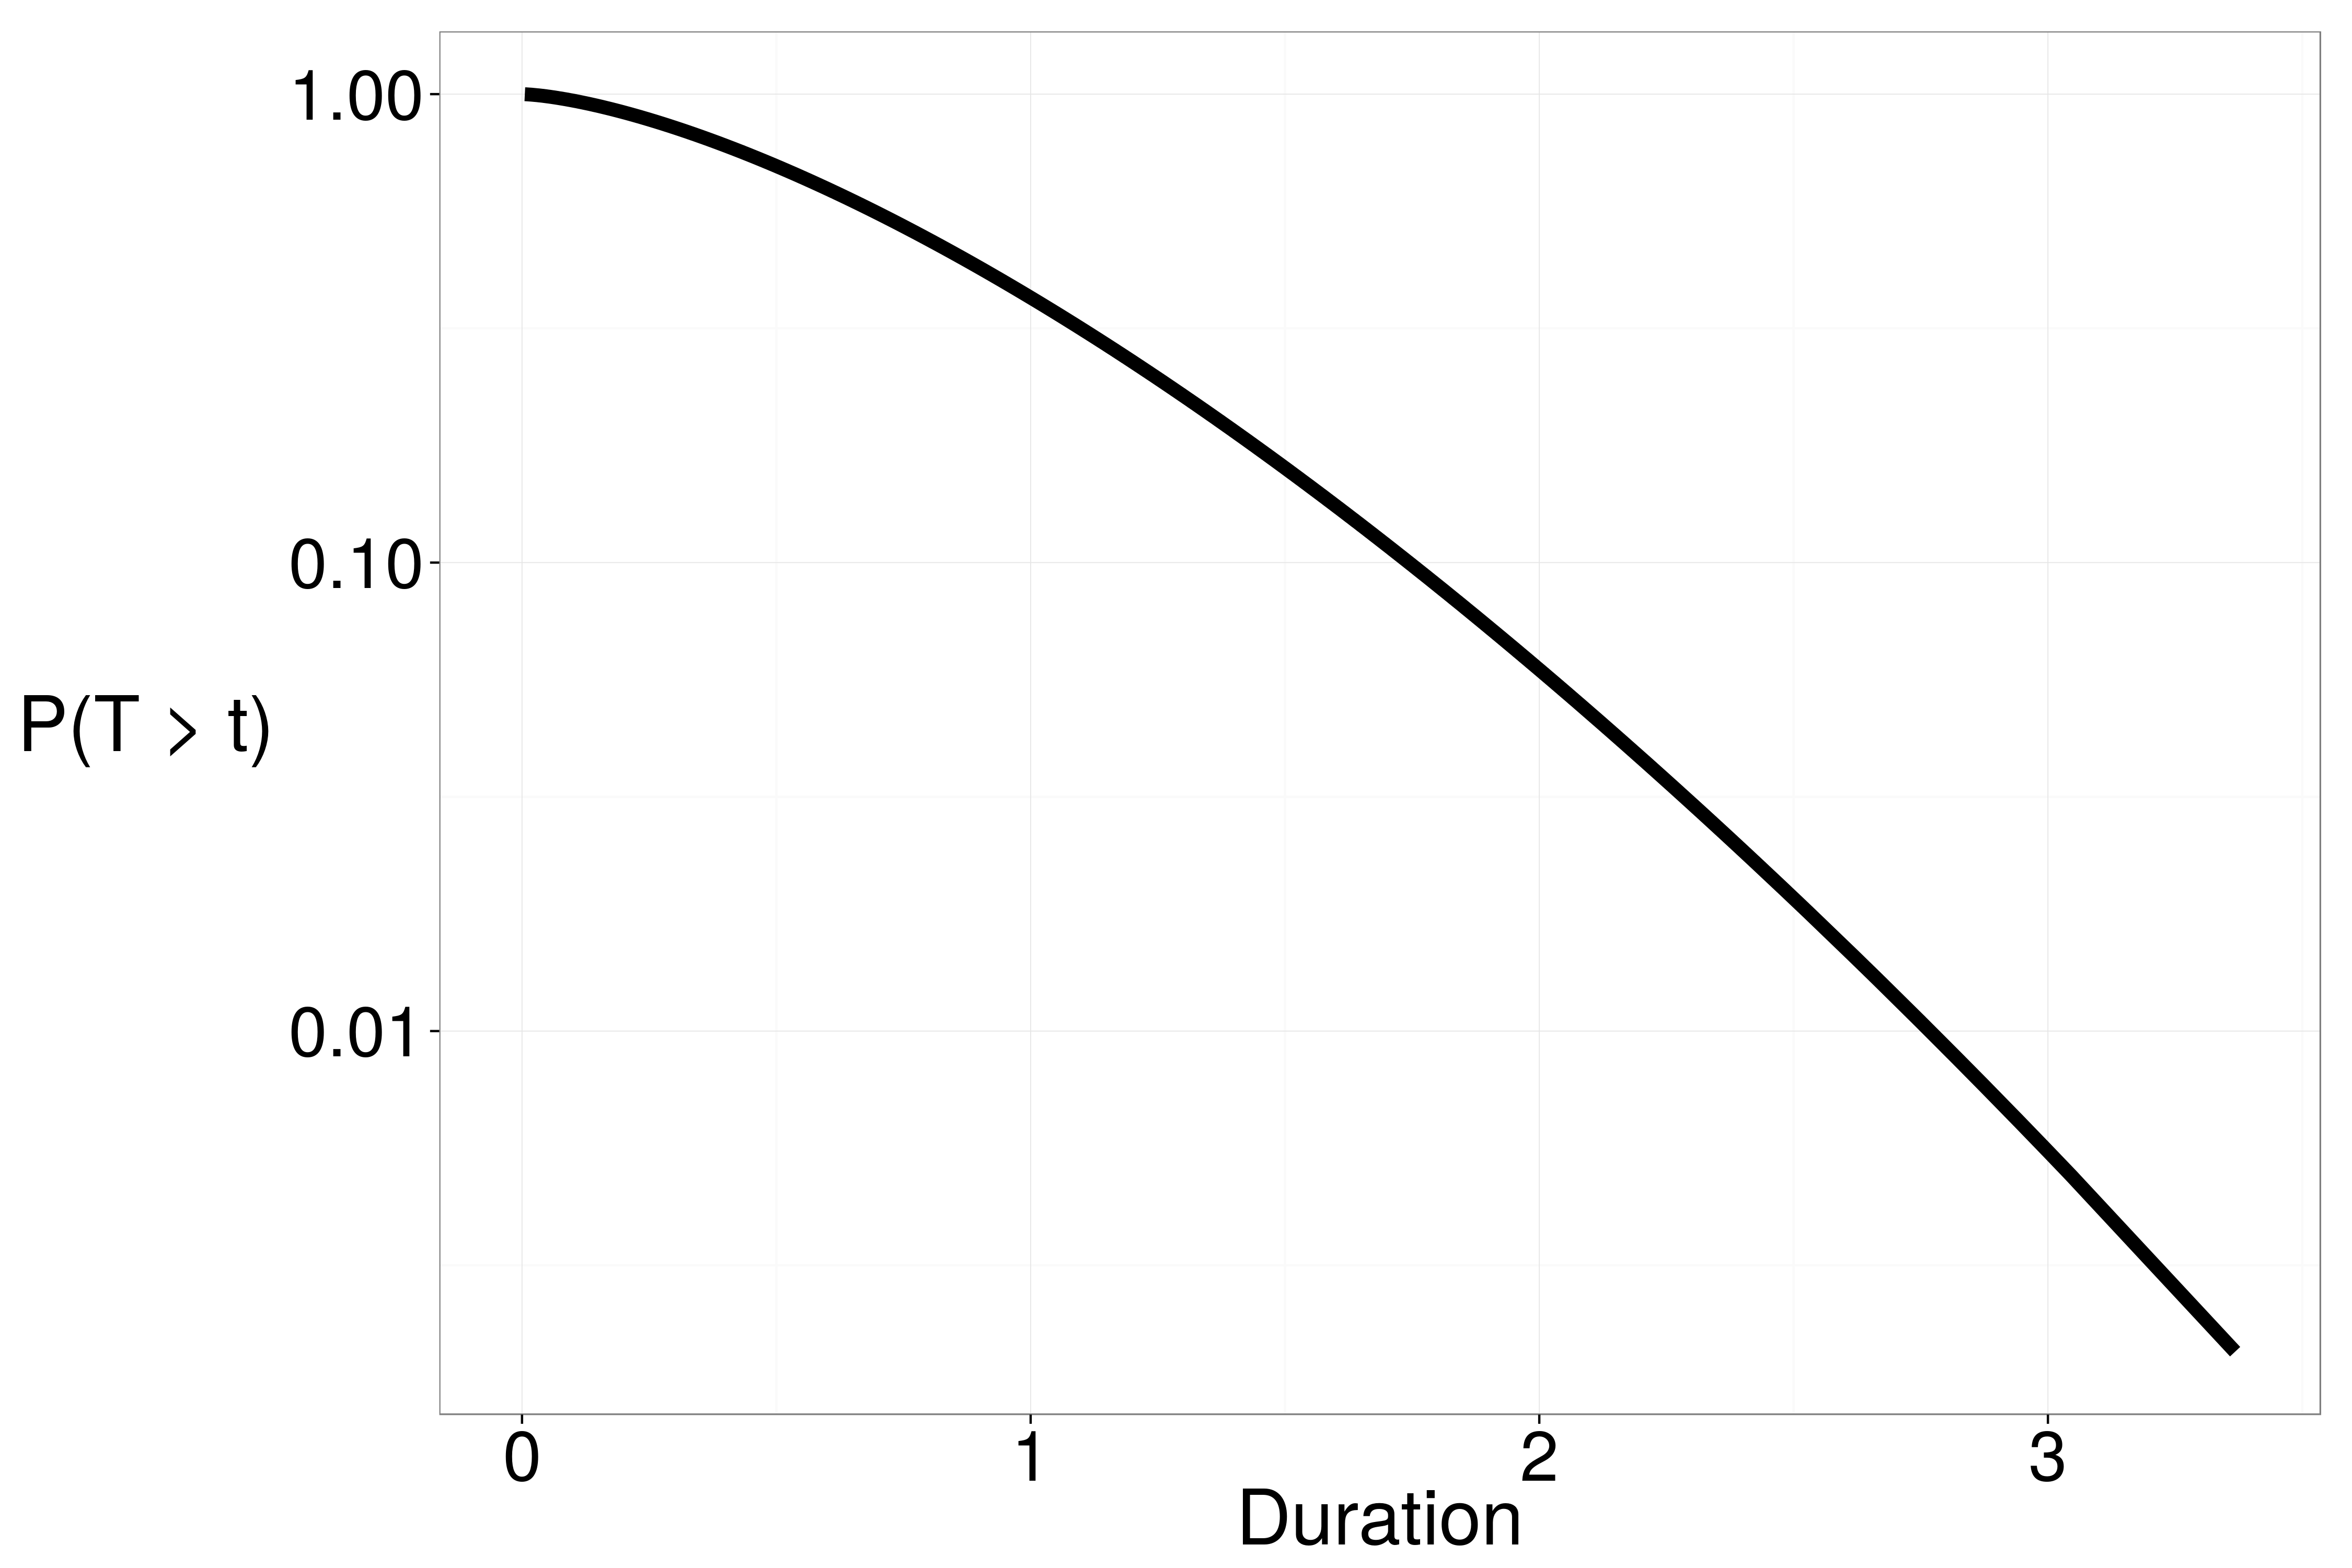
\includegraphics[height = 0.6\textheight, width = 0.5\textwidth, keepaspectratio = true]{figure/sur_acc}
    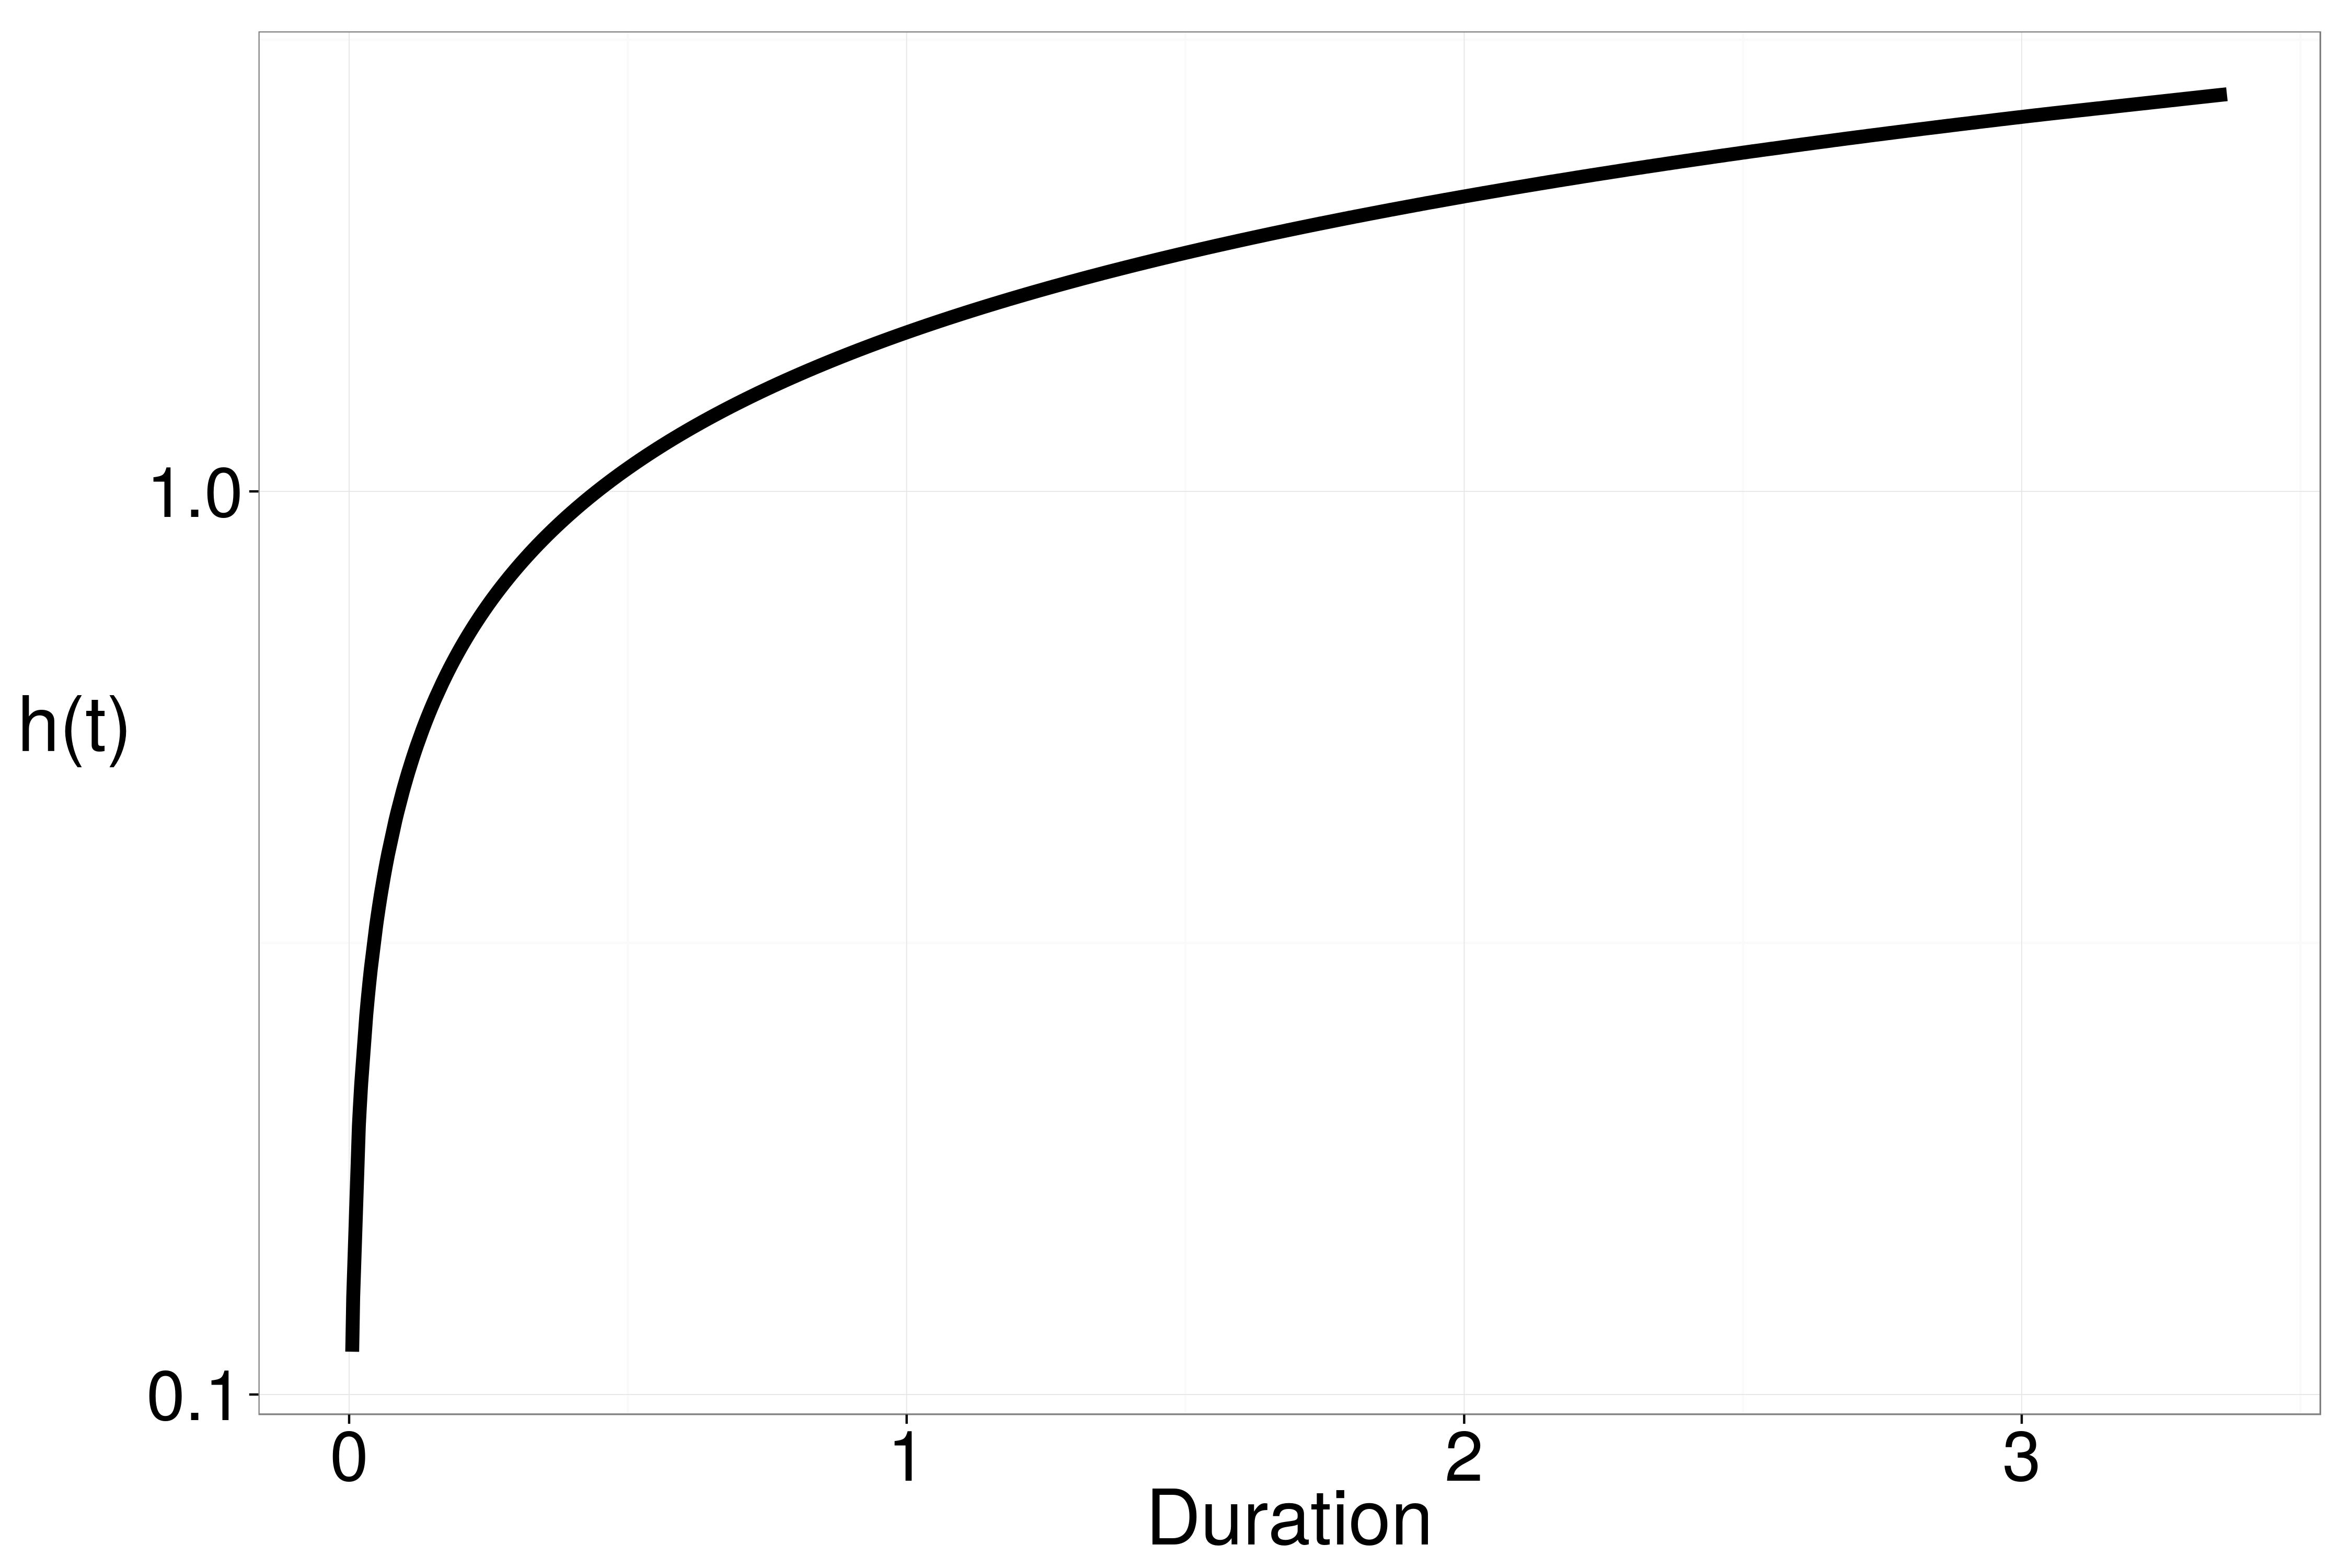
\includegraphics[height = 0.6\textheight, width = 0.5\textwidth, keepaspectratio = true]{figure/haz_acc}
  \end{center}
\end{frame}


\begin{frame}
  \frametitle{Bayesian model structure}
  \begin{center}
    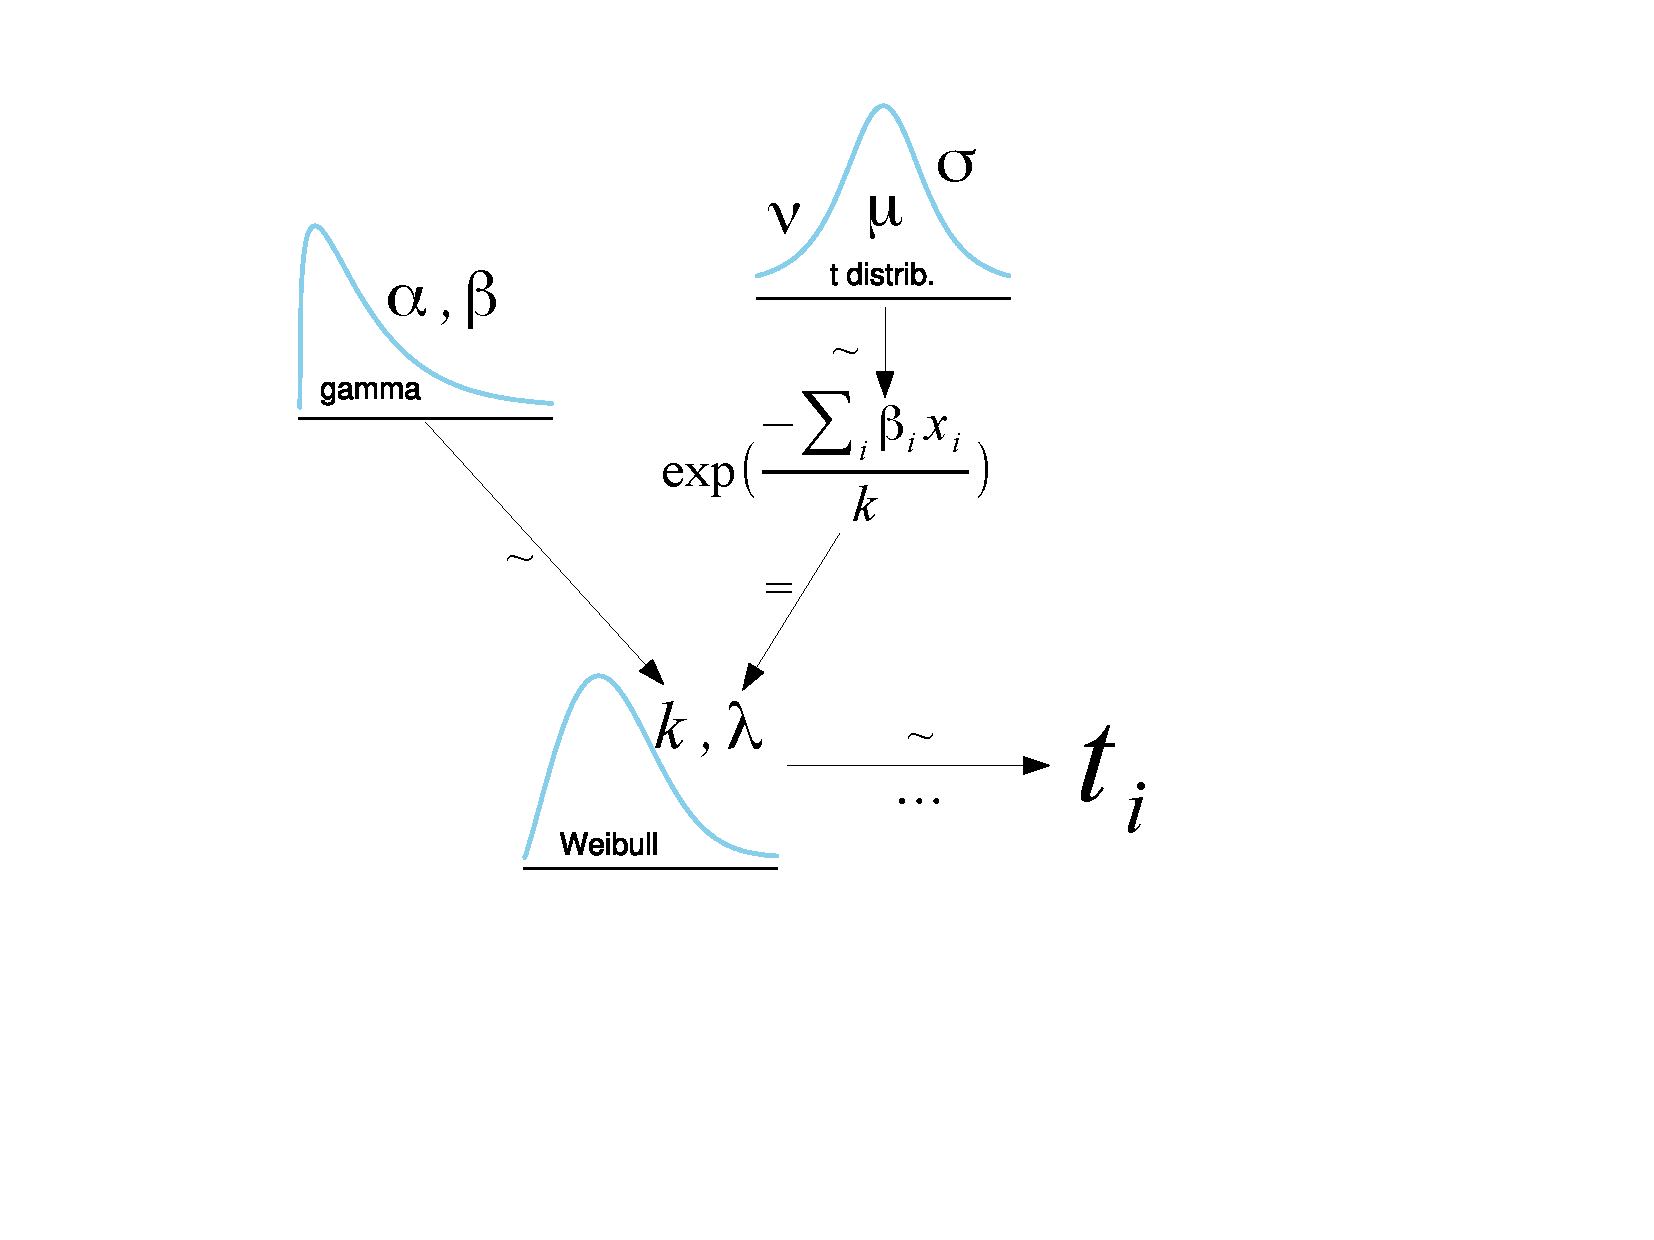
\includegraphics[height = 0.8\textheight, width = \textwidth, keepaspectratio = true]{figure/surv_rev}
  \end{center}
\end{frame}


\begin{frame}
  \frametitle{Parameter marginal posteriors}
  \begin{center}
    For all but \(k\), if farther to \alert{left} then \(\uparrow\) trait \(\propto\) \(\uparrow\) duration.
    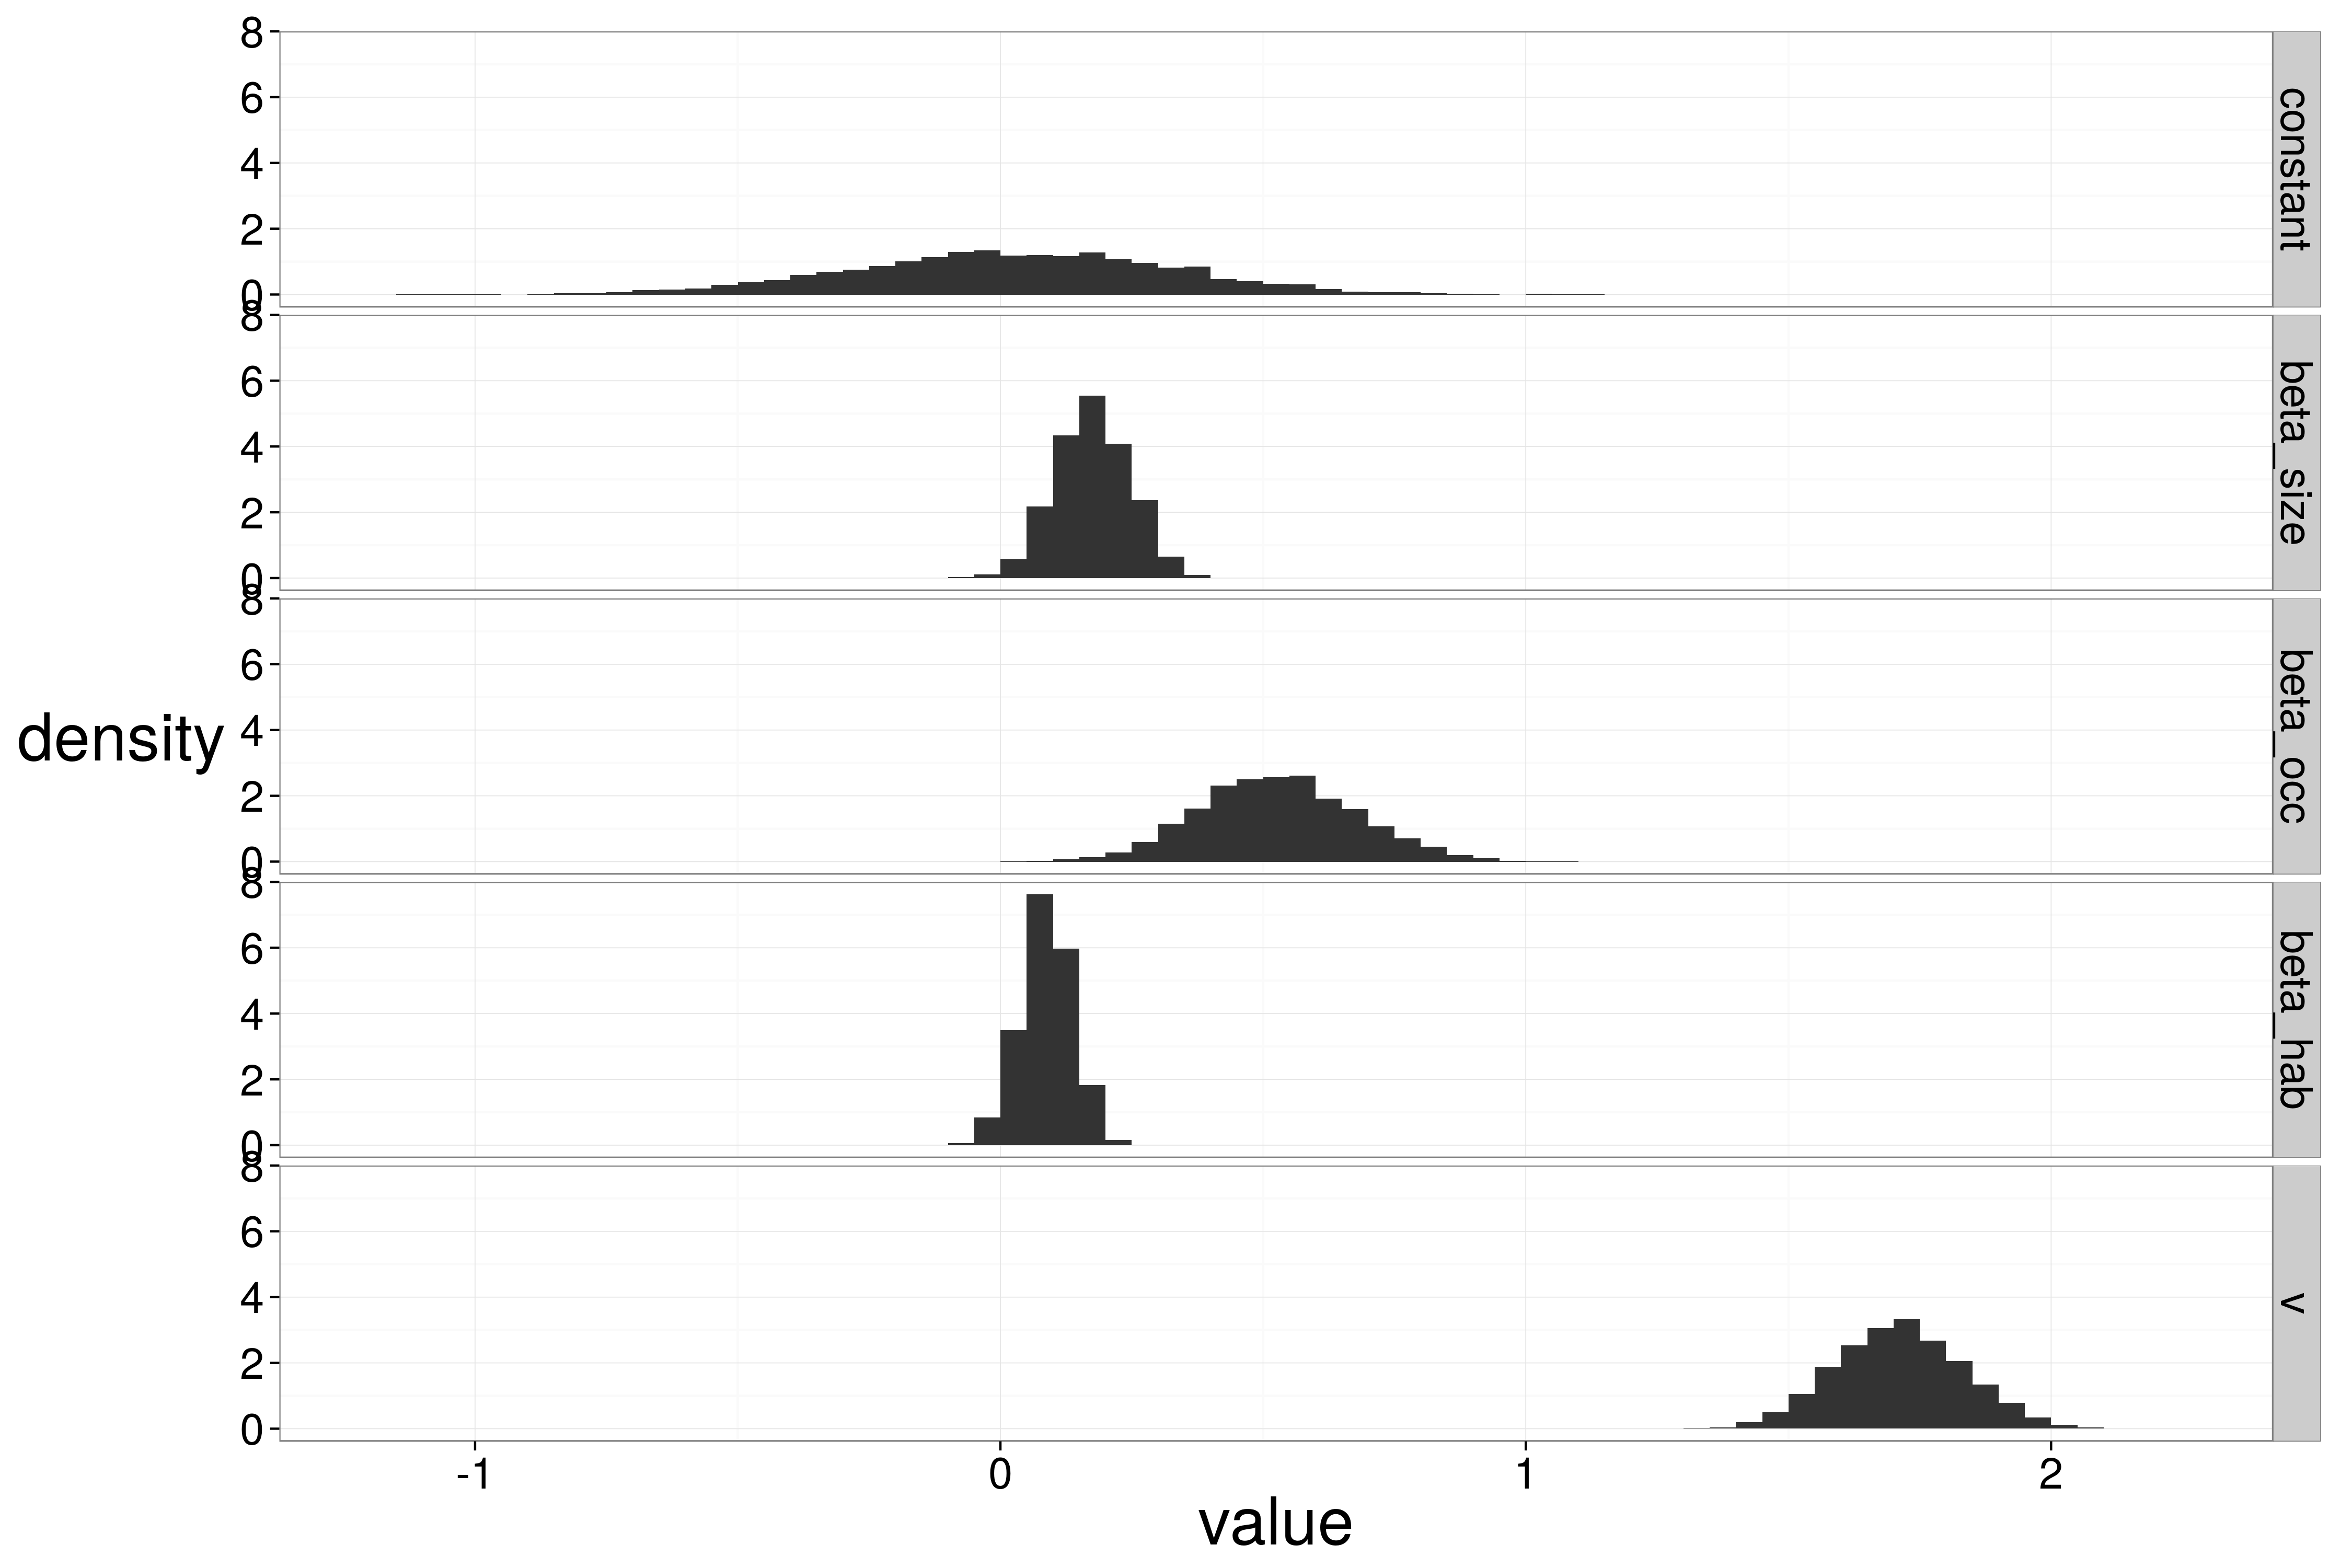
\includegraphics[height = 0.7\textheight, width = \textwidth, keepaspectratio = true]{figure/wei_post}
  \end{center}
\end{frame}

\begin{frame}
  \frametitle{Estimated versus observed: distribution}
  \begin{center}
    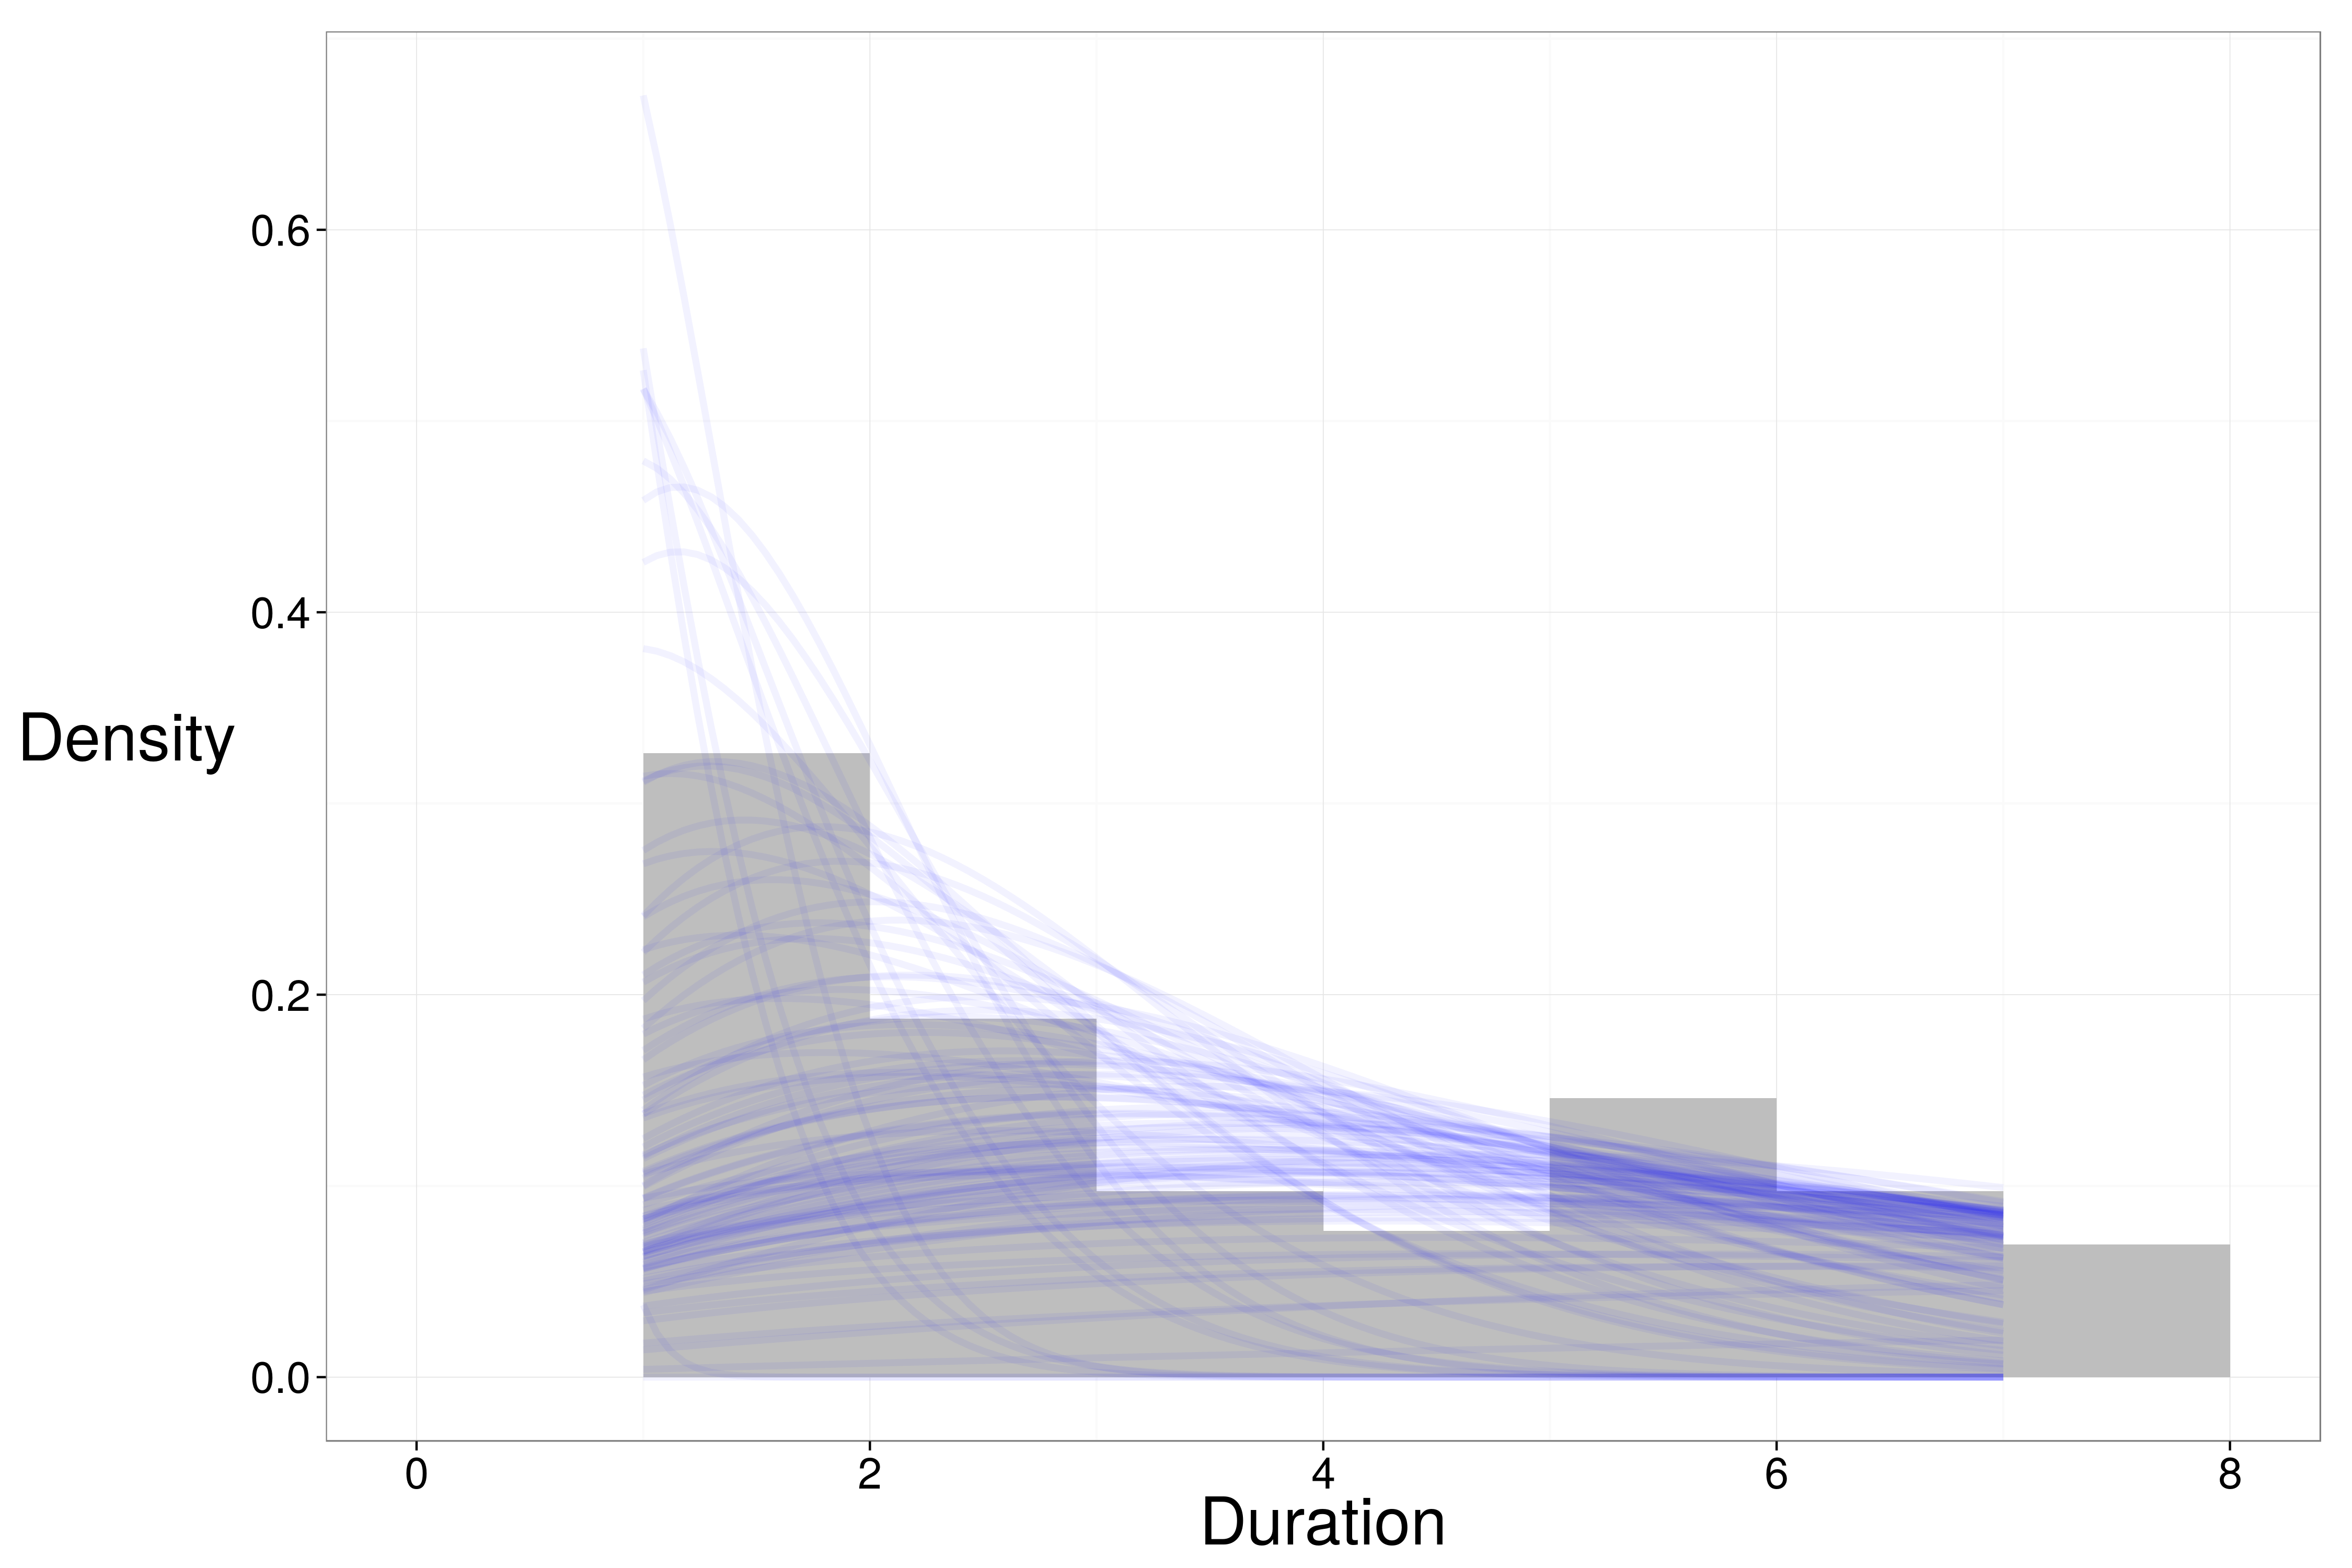
\includegraphics[height = 0.8\textheight, width = \textwidth, keepaspectratio = true]{figure/wei_dur_post}
  \end{center}
\end{frame}

\begin{frame}
  \frametitle{Estimated versus observed: mean duration}
  \begin{center}
    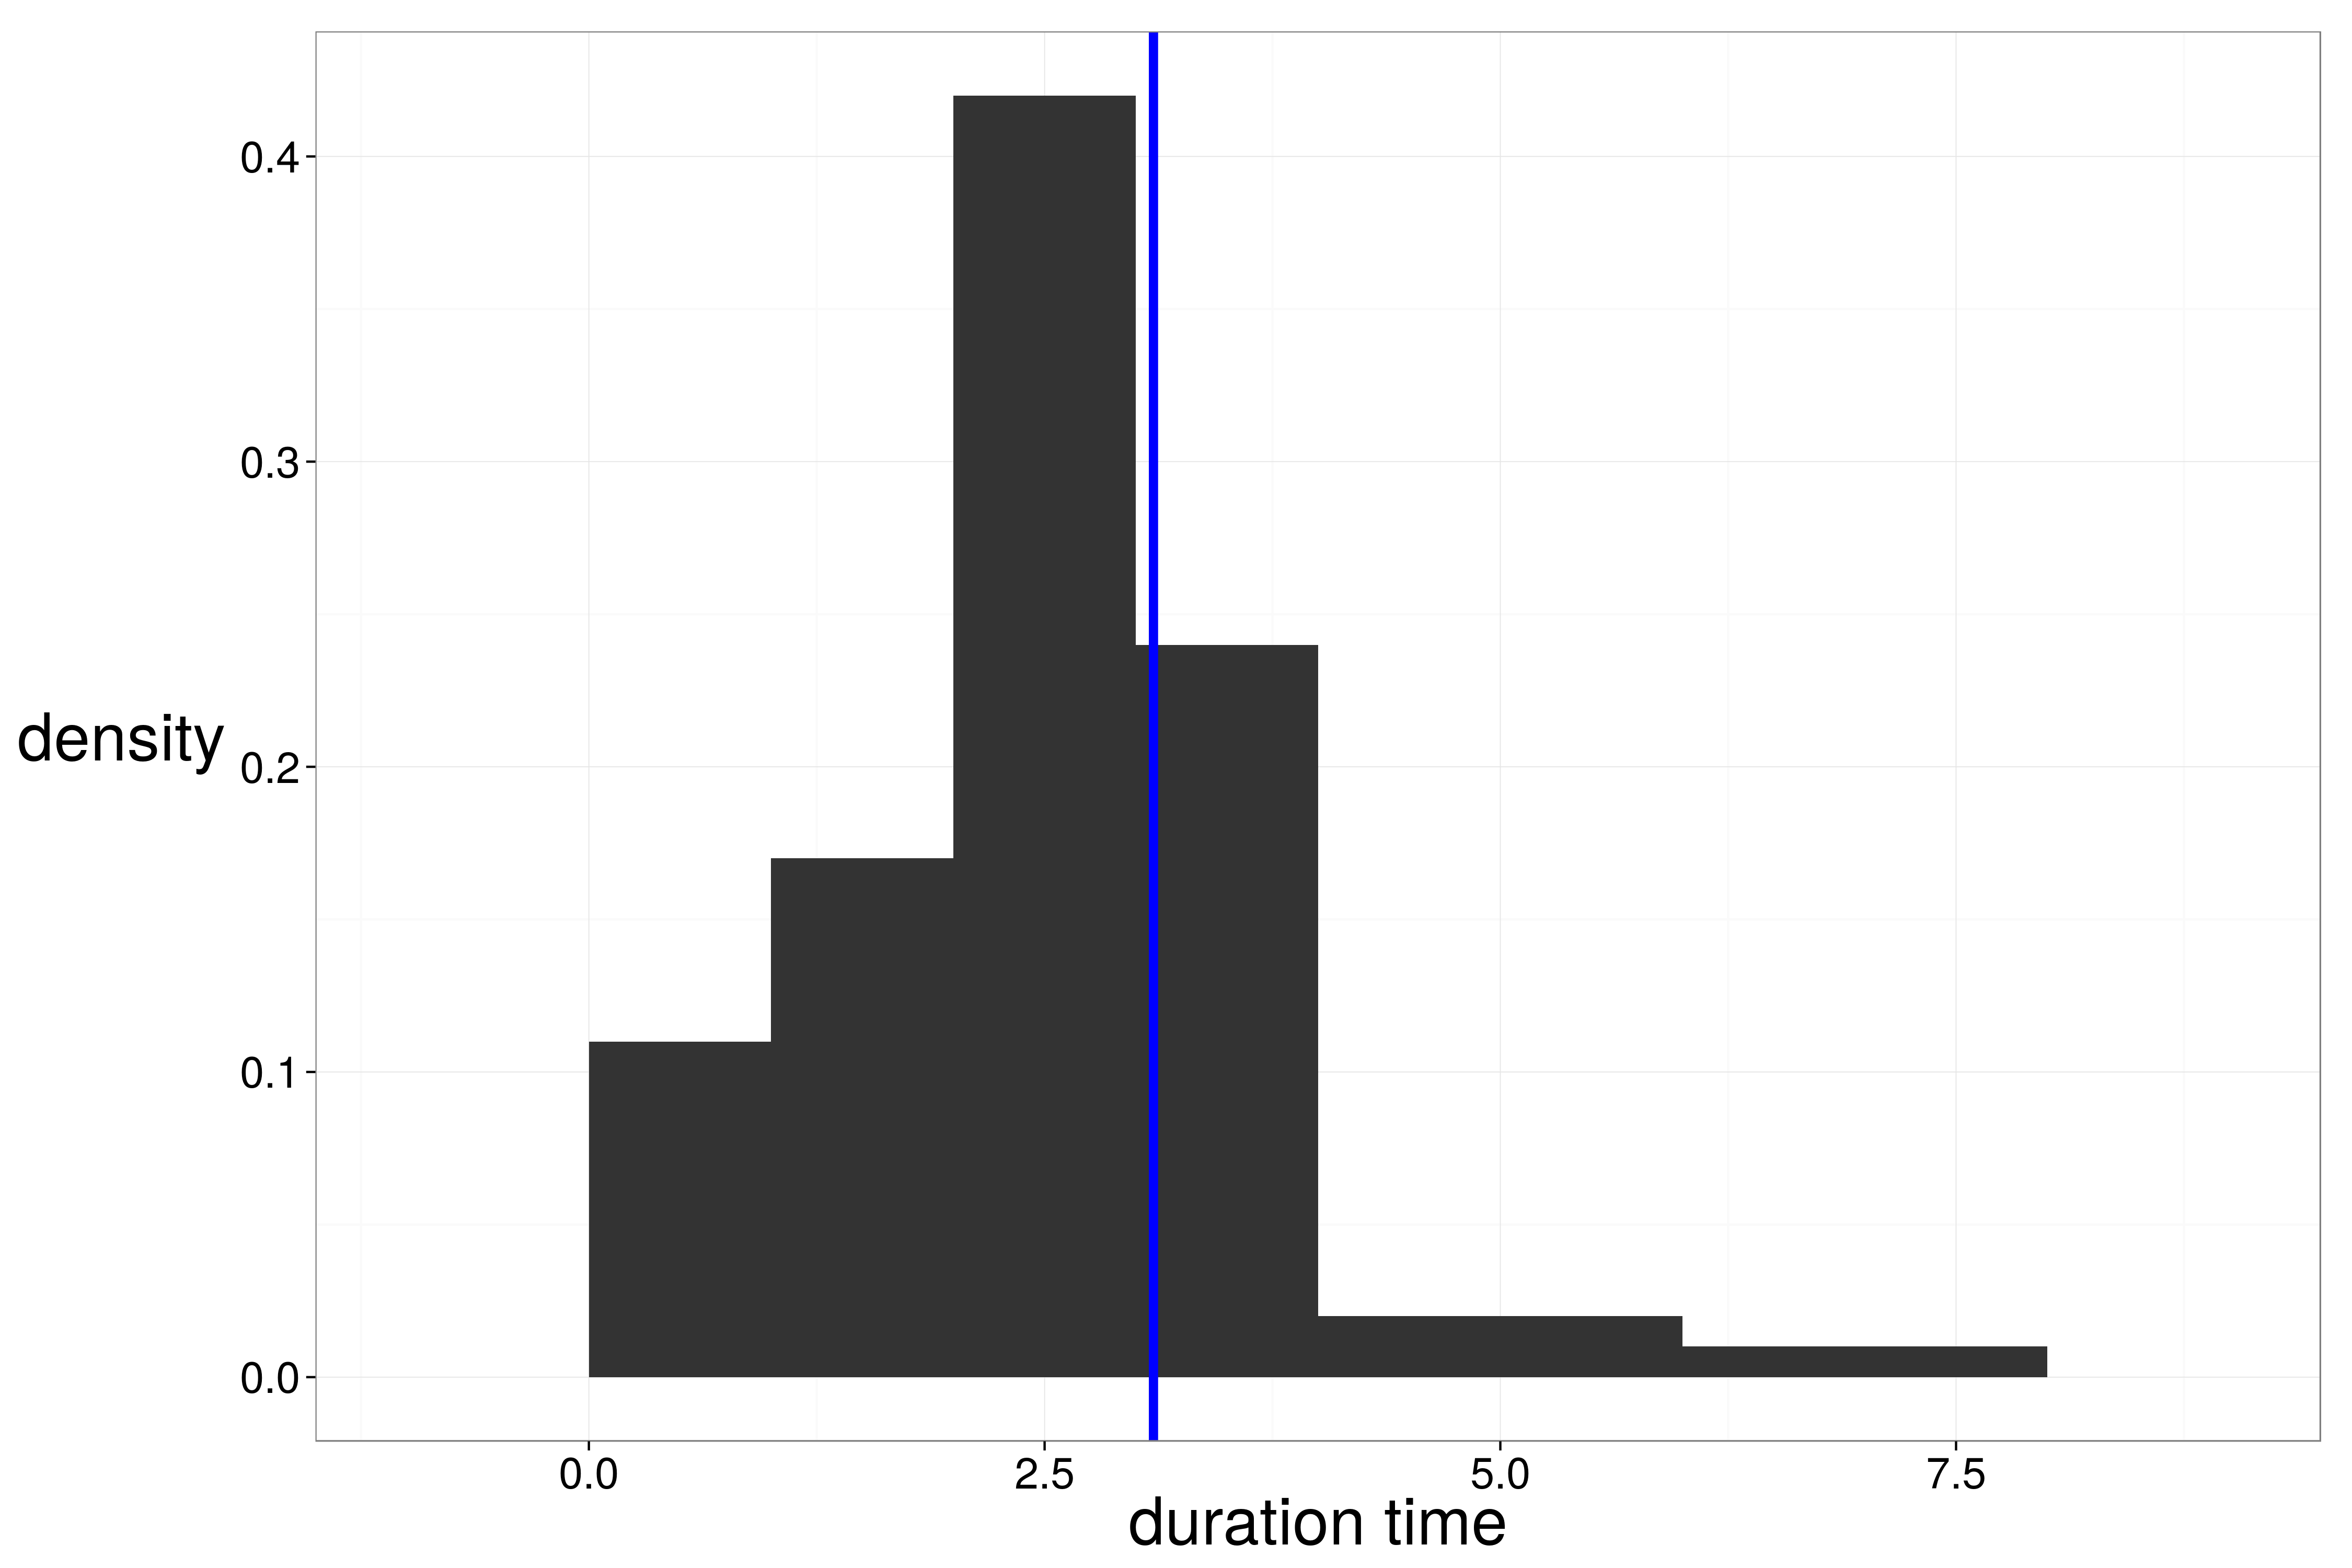
\includegraphics[height = 0.8\textheight, width = \textwidth, keepaspectratio = true]{figure/wei_mean_ppc}
  \end{center}
\end{frame}

\begin{frame}
  \frametitle{Estimated versus observed: quantiles}
  \begin{center}
    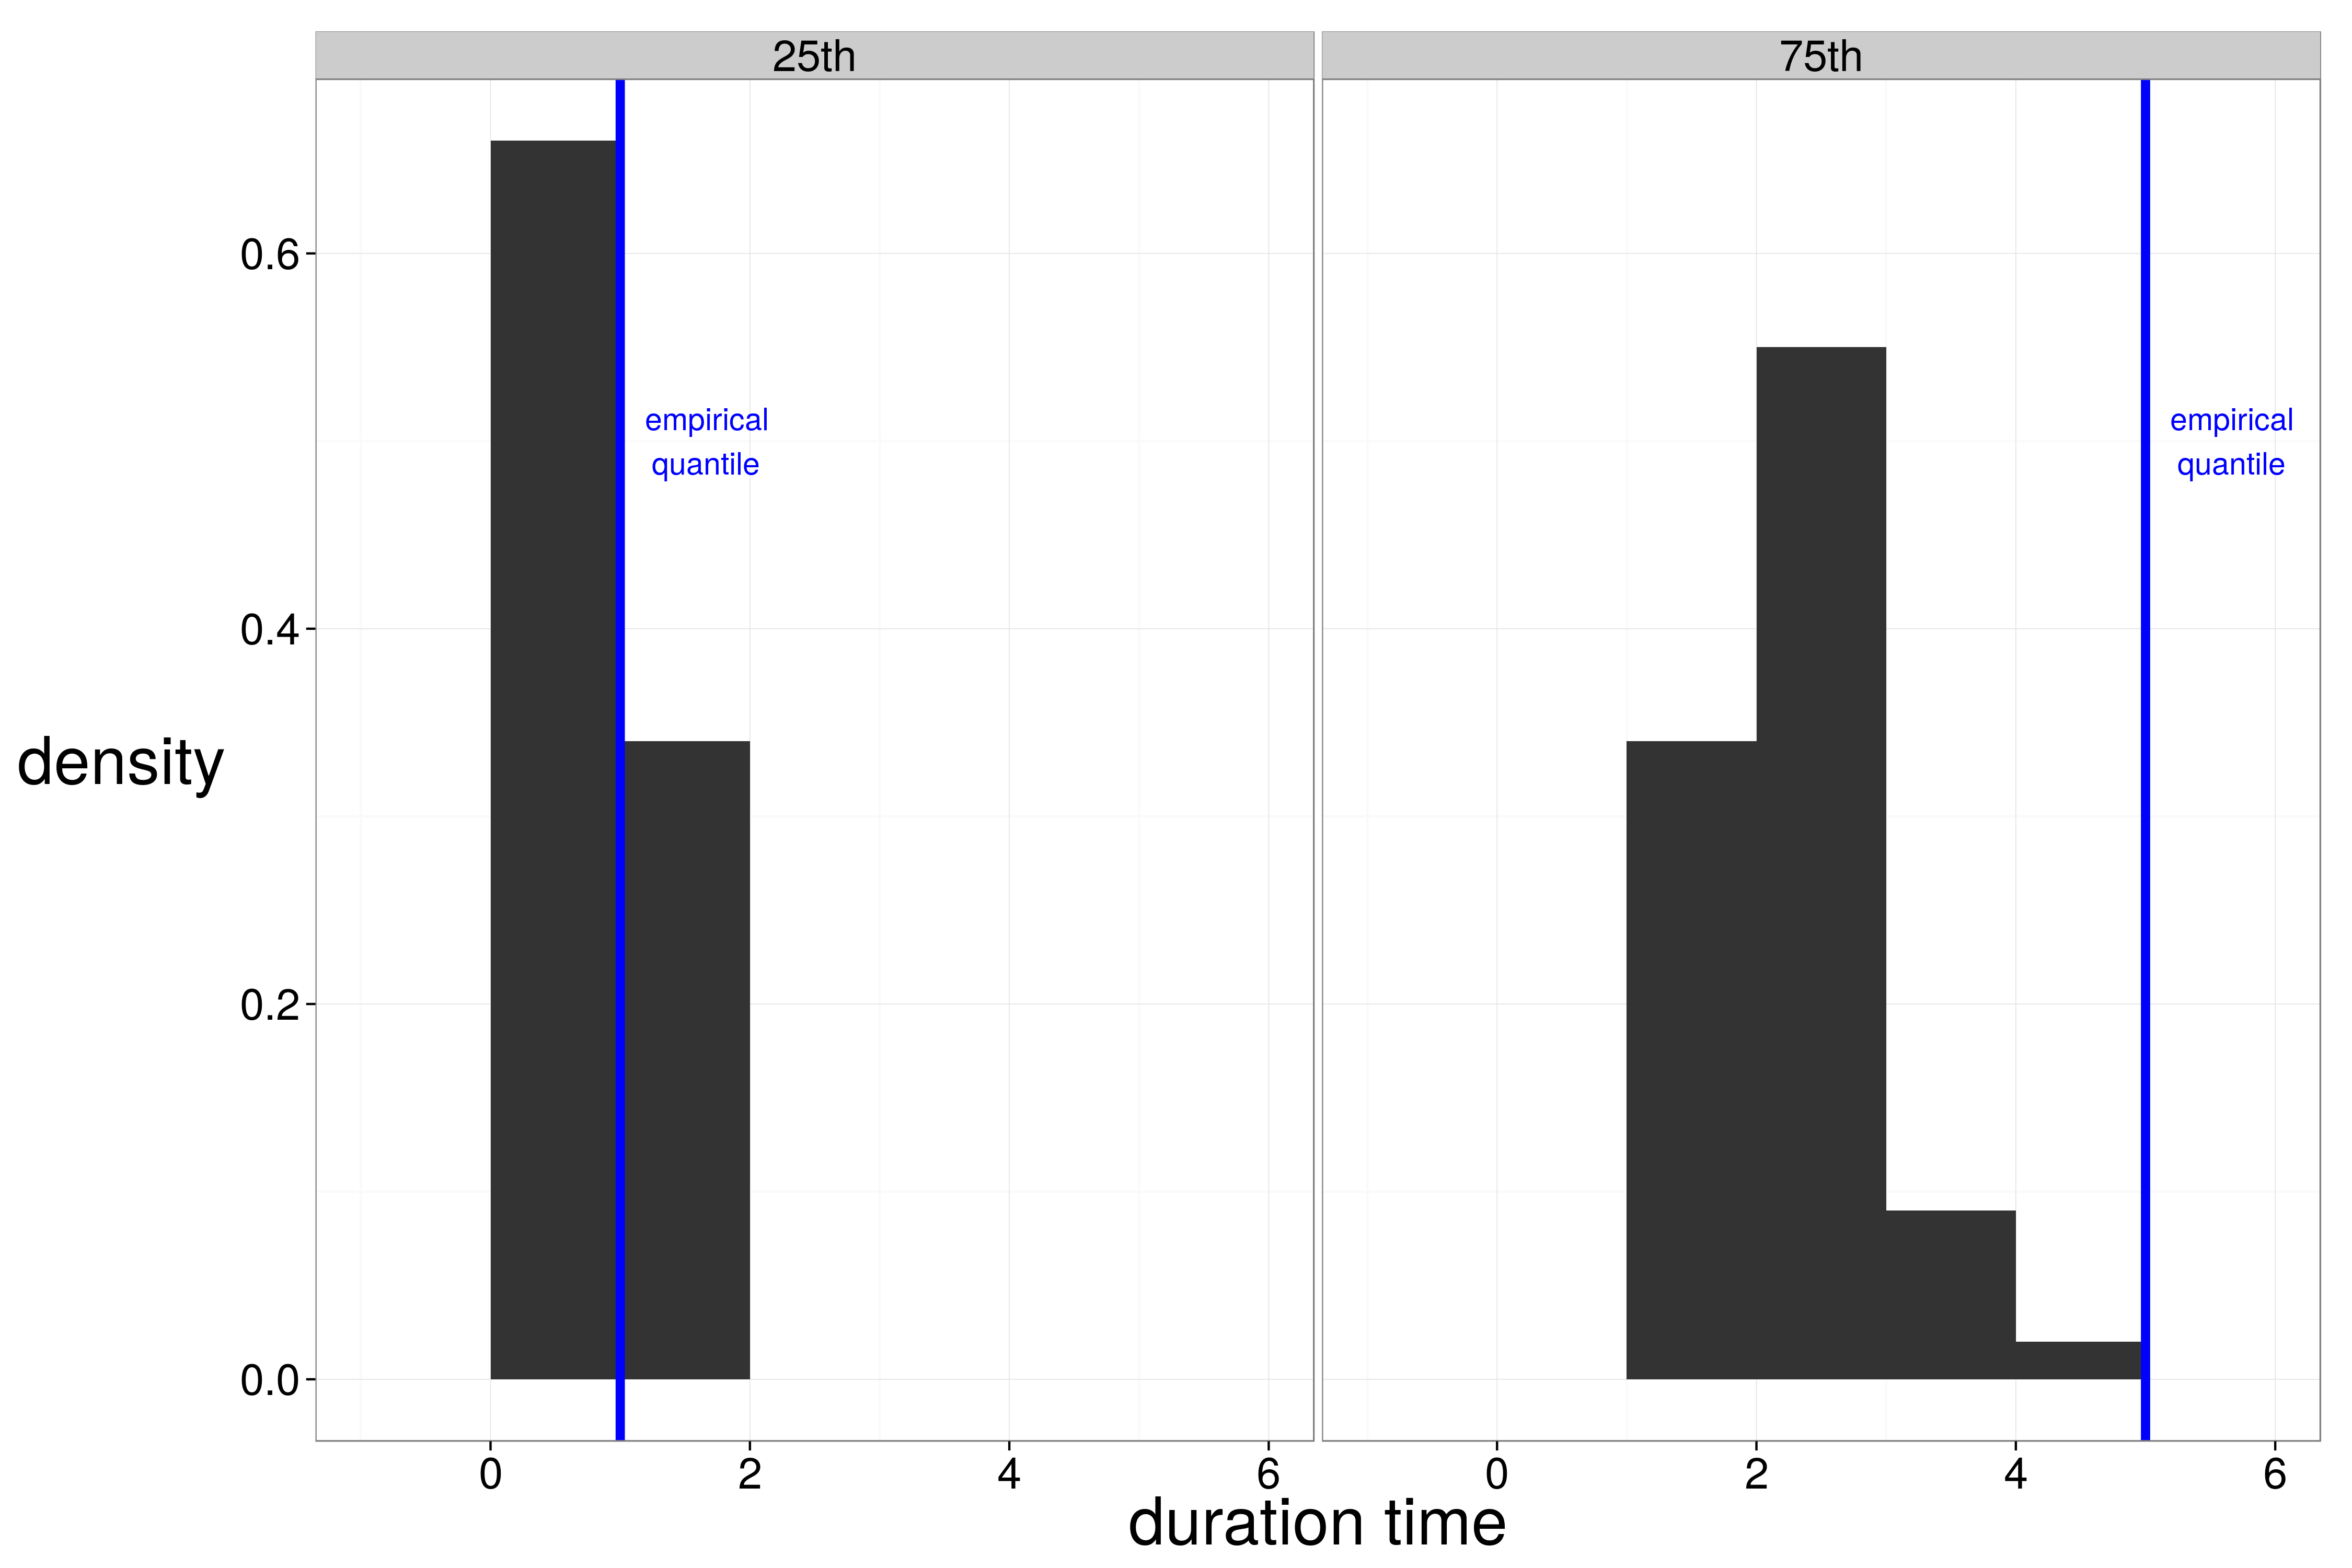
\includegraphics[height = 0.8\textheight, width = \textwidth, keepaspectratio = true]{figure/wei_quant_ppc}
  \end{center}
\end{frame}

\begin{frame}
  \frametitle{State of knowledge}

  \begin{block}{Preliminary conclusions}
    Little evidence for age-independent pattern.

    Occupancy has largest effect. 
    
    P(carbonate \(\mid\) occurrences) \(\approx\) no effect.
  \end{block}
\end{frame}

\begin{frame}
  \frametitle{Modeling improvements}

  \begin{alertblock}{Major roadblock}
    \alert{\uppercase{heavy right tail}}
  \end{alertblock}

  \bigskip

  \begin{itemize}
    \item sampling distribution
      \begin{itemize}
        \item three-parameter Weibull
        \item mixture of distributions
      \end{itemize}
    \item different priors
    \item non-linear/heterogeneous variance
    \item fossil sampling effect
  \end{itemize}
\end{frame}

%\begin{frame}
%  \frametitle{Data set} % replace this text with an image
%  \begin{itemize}
%    \item New Zealand record (FRED)
%    \item improved paleoenvironment reconstructions
%    \item affixing strategy information
%  \end{itemize}
%\end{frame}

\begin{frame}
  \frametitle{Remember\dots}
  Analysis is a narrative

  \bigskip

  \begin{itemize}
    \item fit model
    \item evaluate model
    \item improve model/include more information
  \end{itemize}
\end{frame}


\begin{frame}
  \frametitle{Acknowledgements}
  \begin{columns}
    \begin{column}{0.4\textwidth}
      \begin{itemize}
        \item Advising
          \begin{itemize}
            \item Kenneth D. Angielczyk, Michael J. Foote, P. David Polly, Richard H. Ree
          \end{itemize}

        \item Discussion 
          \begin{itemize}
            \item David Bapst, Marites Villarosa Garcia, Gene Hunt, Nadia Pierrehumbert
          \end{itemize}
      \end{itemize}
    \end{column}
    \begin{column}{0.6\textwidth}
      
\includegraphics[height = 0.3\textheight, keepaspectratio = true]{figure/chicago} 
      
\includegraphics[width = 0.4\textwidth, keepaspectratio = true]{figure/field}

      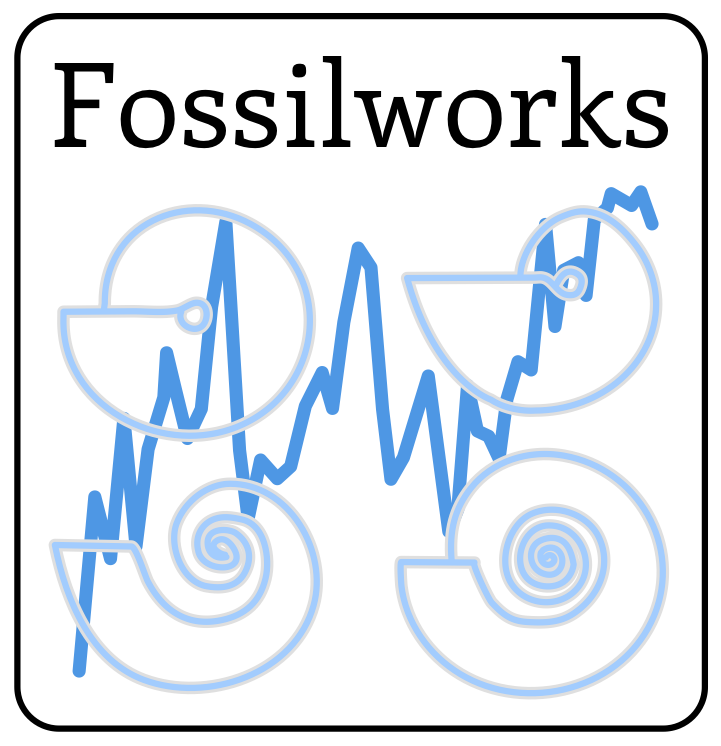
\includegraphics[height = 0.3\textheight, width = 0.5\textwidth, keepaspectratio = true]{figure/fossilworks}
      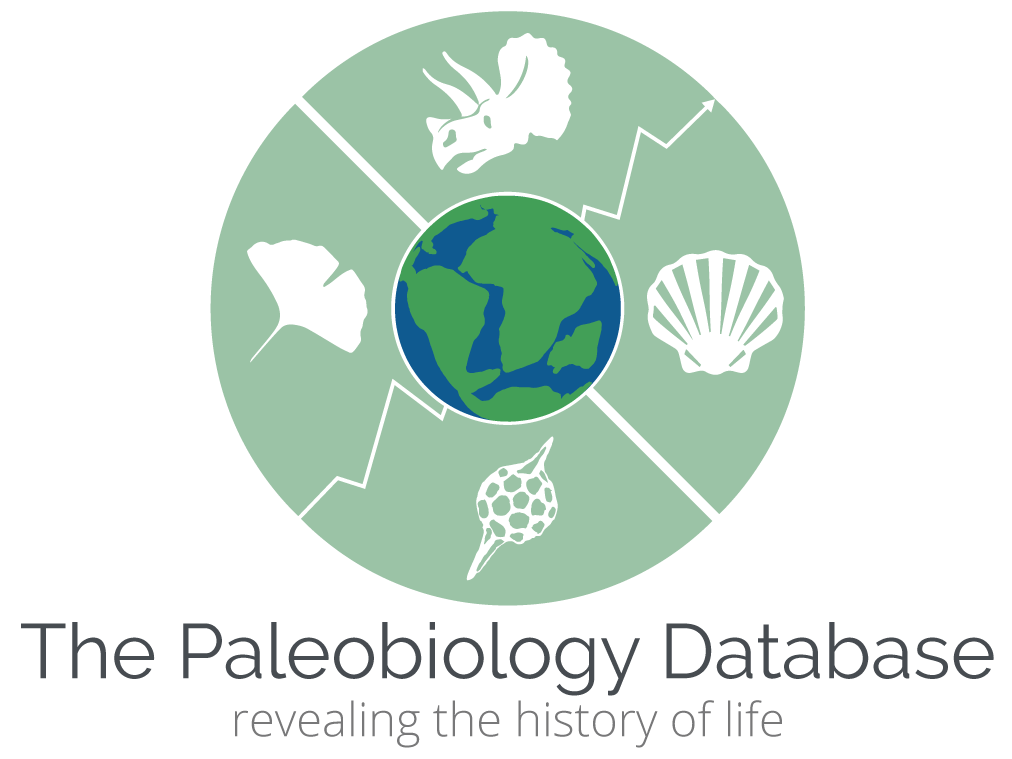
\includegraphics[width = 0.5\textwidth, keepaspectratio = true]{figure/paleodb}

    \end{column}
  \end{columns}
\end{frame}


\end{document}
